\documentclass[aspectratio=169,10pt]{beamer}
\usetheme{mekatronik}
\setday{4}{Servo Systems: Drives, FOC, Loops}
\title[Day 4 -- Servo Drives, FOC and Control Loops]{Servo Systems: Drives, FOC, Control Loops, Tuning and Compensation}
\subtitle{3.2 PWM \& limits \textbullet\ 3.3 Field-oriented control \textbullet\ 3.4 Cascade loops \textbullet\ 3.5 Tuning \& bandwidth \textbullet\ 3.6 Disturbance compensation}
\author{Mechatronics Training Programme}
\institute{Theoretical Course Series}
\date{Day 4 of 5}

% ---- local helpers -------------------------------------------------
\tikzset{
  blk/.style={draw=mkBlue,fill=mkPale,rounded corners=1.5pt,minimum height=7mm,minimum width=12mm,font=\scriptsize,align=center,line width=.6pt},
  blko/.style={blk,draw=mkOrange,fill=mkCream},
  sumn/.style={draw=mkBlue,circle,inner sep=0pt,minimum size=4mm,fill=white,line width=.6pt},
  sig/.style={-{Latex[length=2mm]},mkNavy,line width=.6pt},
  fb/.style={-{Latex[length=2mm]},mkMid,line width=.6pt},
  ff/.style={-{Latex[length=2mm]},mkOrange,line width=.7pt,dashed},
  lab/.style={font=\tiny,text=mkNavy},
}
\newcommand{\src}[1]{\par\vfill\hfill{\color{mkGray}\fontsize{6}{7}\selectfont #1}}
\pgfplotsset{every axis/.append style={label style={font=\scriptsize}}}

\begin{document}

\begin{frame}[plain]\titlepage\end{frame}

% =====================================================================
\begin{frame}[t]{Agenda and learning objectives}
\begin{columns}[T,onlytextwidth]
\column{.54\textwidth}
\footnotesize
\begin{tabularx}{\linewidth}{@{}l X r@{}}
\toprule
\textbf{Code} & \textbf{Session} & \textbf{Net time}\\
\midrule
3.2 & (cont.) PWM, modulation range, dead time, limits & 0.5 h\\
3.3 & Field-oriented control of the PMSM & 1.5 h\\
3.4 & Current, velocity and position loops; trajectories & 1.5 h\\
3.5 & Loop tuning and bandwidth & 1.0 h\\
3.6 & Disturbances and compensation & 0.5 h\\
\midrule
 & \textbf{Total} (+ 10-min breaks about every hour) & \textbf{5.0 h}\\
\bottomrule
\end{tabularx}\\[2mm]
\begin{notebox}
\textbf{Reference motor used all day} (surface-mounted PMSM servo):
$p=4$, $R=\SI{0.5}{\ohm}$, $L_d=L_q=\SI{3}{mH}$, $\psi_\text{PM}=\SI{0.12}{Vs}$,
$k_t=\tfrac32 p\psi_\text{PM}=\SI{0.72}{Nm/A}$, $J_m=\SI{3e-4}{kg\,m^2}$, load inertia ratio 3,
$V_\text{dc}=\SI{325}{V}$, $\hat I_\text{max}=\SI{20}{A}$, $f_\text{PWM}=f_s=\SI{16}{kHz}$.
\end{notebox}
\column{.43\textwidth}
\begin{keybox}[By the end of the day you can \ldots]
\scriptsize
\checkitem\ compute SVPWM dwell times and the limit $V_\text{dc}/\sqrt3$\\
\checkitem\ transform $abc \to \alpha\beta \to dq$; write the PMSM $dq$ model\\
\checkitem\ explain the FOC structure, MTPA and field weakening\\
\checkitem\ design PI current/velocity loops (TO / SO)\\
\checkitem\ size bandwidths; quantify the phase cost of delays\\
\checkitem\ generate motion profiles; cancel following error by feedforward\\
\checkitem\ explain disturbance observers and cogging compensation
\end{keybox}
\end{columns}
\end{frame}

% =====================================================================
\section{3.2 (cont.) Motor Driving: PWM, Voltage and Current Limits}
% =====================================================================

\begin{frame}[t]{The two-level voltage-source inverter and carrier-based sinusoidal PWM}
\begin{columns}[T,onlytextwidth]
\column{.40\textwidth}
\centering
\begin{circuitikz}[scale=.7,transform shape,line width=.5pt]
\draw (0,0) -- (6,0);  \draw (0,4) -- (6,4);
\draw (0,4) to[C,l_=$C_\text{dc}$] (0,0);
\node[anchor=east,font=\scriptsize] at (-.4,2.0) {$V_\text{dc}$};
\foreach \x/\n in {1.6/a,3.4/b,5.2/c}{
  \draw (\x,4) to[Tnigbt,mirror] (\x,2) to[Tnigbt,mirror] (\x,0);
  \draw (\x,2) to[short,*-o] (\x+.6,2) node[right,font=\scriptsize]{$\n$};
}
\node[font=\tiny,mkGray] at (1.0,3.0) {$S_a$};
\node[font=\tiny,mkGray] at (1.0,1.0) {$\bar S_a$};
\end{circuitikz}\\[1mm]
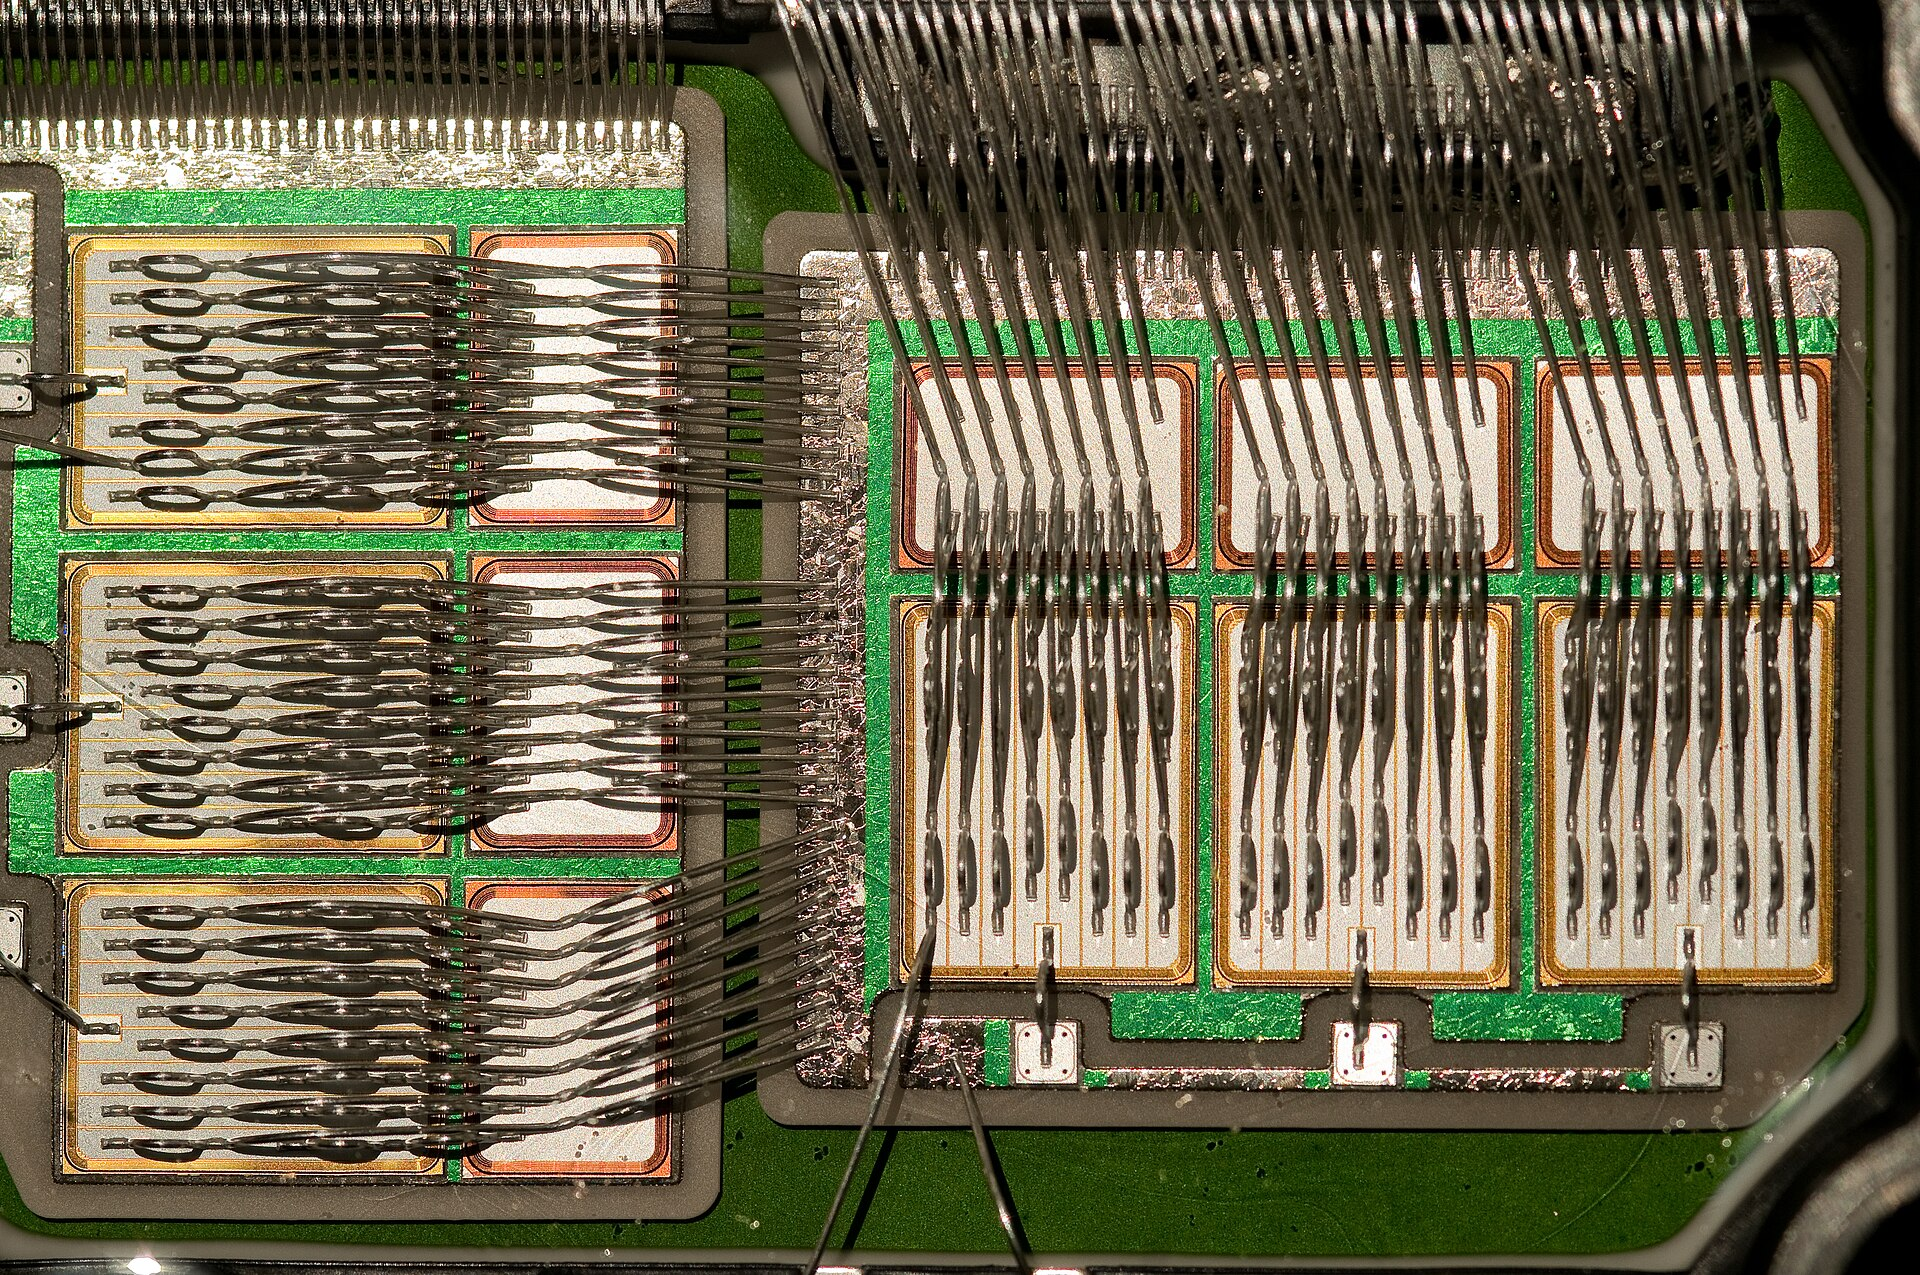
\includegraphics[width=.95\linewidth,height=2.5cm,keepaspectratio]{../figures/d4_igbt_module.jpg}\\
\credit{Pslawinski, CC BY-SA 3.0, via Wikimedia Commons}
\column{.58\textwidth}
\begin{tikzpicture}
\begin{groupplot}[group style={group size=1 by 3,vertical sep=2mm,xticklabels at=edge bottom},
  mkplot,width=8.6cm,xmin=0,xmax=360,xtick={0,90,180,270,360},
  every axis plot/.append style={line width=.5pt},grid=none,yticklabel style={font=\tiny}]
\nextgroupplot[height=2.9cm,ymin=-1.1,ymax=1.1,ylabel={$v^*$, carrier},ytick={-1,0,1}]
\addplot[mkSky,line width=.3pt] table[x=th,y=car]{data/spwm.dat};
\addplot[mkBlue,thick] table[x=th,y=va]{data/spwm.dat};
\addplot[mkOrange,thick] table[x=th,y=vb]{data/spwm.dat};
\nextgroupplot[height=2.1cm,ymin=-.2,ymax=2.4,ytick={0.5,1.8},yticklabels={$S_a$,$S_b$}]
\addplot[mkBlue] table[x=th,y=Sa]{data/spwm.dat};
\addplot[mkOrange] table[x=th,y expr=\thisrow{Sb}+1.3]{data/spwm.dat};
\nextgroupplot[height=2.3cm,ymin=-1.3,ymax=1.3,ytick={-1,0,1},ylabel={$v_{ab}/V_\text{dc}$},xlabel style={yshift=1mm},xlabel={$\omega_1 t$ (deg)}]
\addplot[mkMid] table[x=th,y=vab]{data/spwm.dat};
\addplot[mkOrange,thick,domain=0:360,samples=90] {0.8*0.866*sin(x+30)};
\end{groupplot}
\end{tikzpicture}\\[-1mm]
\scriptsize Compare $v_a^*=m\sin\omega_1 t$ with a triangle carrier ($m=0.8$, $m_f=15$): leg $a$ ON when $v_a^*>$ carrier.
Pole voltage average $\bar v_{aN}=\tfrac{V_\text{dc}}{2}(1+v_a^*)$ $\Rightarrow$ fundamental phase amplitude $\hat V_1=m\,V_\text{dc}/2$.
\end{columns}
\end{frame}

% ---------------------------------------------------------------------
\begin{frame}[t]{Zero-sequence injection: third harmonic and min--max (SVPWM-equivalent)}
\begin{columns}[T,onlytextwidth]
\column{.52\textwidth}
\begin{tikzpicture}
\begin{axis}[mkplot,width=7.8cm,height=5.0cm,xmin=0,xmax=360,ymin=-1.3,ymax=1.3,
  xtick={0,60,...,360},xlabel={$\omega_1 t$ (deg)},ylabel={modulating signal (p.u. of $V_\text{dc}/2$)},
  legend style={at={(0.5,1.02)},anchor=south},legend columns=4]
\addplot[mkSky,thick,dashed] table[x=th,y=sine]{data/zeroseq.dat};
\addplot[mkOrange,thick] table[x=th,y=thi]{data/zeroseq.dat};
\addplot[mkBlue,thick] table[x=th,y=svpwm]{data/zeroseq.dat};
\addplot[mkMid,dotted,thick] table[x=th,y=zs]{data/zeroseq.dat};
\addplot[mkRed,thin,domain=0:360] {1};\addplot[mkRed,thin,domain=0:360] {-1};
\legend{pure sine,3rd harm.\ $+\tfrac16$,min--max,$v_0$}
\end{axis}
\end{tikzpicture}\\
\scriptsize All curves for $\hat V_1 = \tfrac{2}{\sqrt3}\tfrac{V_\text{dc}}{2}=V_\text{dc}/\sqrt3$: the pure sine saturates, the injected signals just fit.
\column{.46\textwidth}
\begin{itemize}\small
\item A common-mode term $v_0$ added to all three references \hl{cancels in the line-to-line voltages} (isolated star point).
\item Third-harmonic injection: $v_x^*= m[\sin\theta_x+\tfrac16\sin3\theta]$
\item Min--max injection: $v_0=-\tfrac12[\max(v^*)+\min(v^*)]$ -- identical average voltages to centred SVPWM.
\end{itemize}
\begin{eqbox}\small\centering
$\hat V_{1,\text{max}}$:\ \ $V_\text{dc}/2$ (SPWM) $\ \rightarrow\ V_\text{dc}/\sqrt3$ (THI, SVPWM)\\
$= +15.5\,\%$ linear voltage range
\end{eqbox}
\begin{notebox}
Beyond: \term{overmodulation} up to six-step ($\hat V_1=\tfrac{2}{\pi}V_\text{dc}$), with low-order harmonics and non-linear gain.
\end{notebox}
\end{columns}
\end{frame}

% ---------------------------------------------------------------------
\begin{frame}[t]{Space vectors: the inverter hexagon}
\begin{columns}[T,onlytextwidth]
\column{.48\textwidth}
\centering
\begin{tikzpicture}[scale=1.55]
  \def\r{1.333}
  % sectors shading
  \fill[mkCream!70] (0,0) -- (0:\r) -- (60:\r) -- cycle;
  \draw[mkGray,->] (-1.65,0) -- (1.75,0) node[right,font=\scriptsize]{$\alpha$};
  \draw[mkGray,->] (0,-1.4) -- (0,1.45) node[above,font=\scriptsize]{$\beta$};
  \draw[mkBlue,line width=.9pt] (0:\r) -- (60:\r) -- (120:\r) -- (180:\r) -- (240:\r) -- (300:\r) -- cycle;
  \draw[mkOrange,dashed,line width=.7pt] (0,0) circle (1.1547);
  \foreach \a/\n/\s in {0/1/100,60/2/110,120/3/010,180/4/011,240/5/001,300/6/101}{
    \draw[-{Latex[length=1.6mm]},mkBlue,line width=.8pt] (0,0) -- (\a:\r);
    \node[font=\tiny,fill=white,inner sep=.5pt] at (\a:{\r+.22}) {$\vec v_{\n}$\,[\s]};
  }
  \foreach \a/\k in {30/I,90/II,150/III,210/IV,270/V,330/VI}{\node[font=\tiny\bfseries,mkMid] at (\a:.82) {\k};}
  \node[font=\tiny,fill=white,inner sep=.5pt] at (-.22,-.13) {$\vec v_0,\vec v_7$};
  \draw[-{Latex[length=1.8mm]},mkOrange,line width=1.1pt] (0,0) -- (22:1.0) node[above right,font=\scriptsize,inner sep=1pt]{$\vec v^*$};
  \draw[mkOrange] (.35,0) arc (0:22:.35); \node[font=\tiny,mkOrange] at (11:.48) {$\theta$};
  \node[font=\tiny,mkOrange,align=left,anchor=west] at (-1.85,-1.05) {inscribed circle\\$|\vec v|=V_\text{dc}/\sqrt3$};
  \node[font=\tiny,mkBlue] at (1.25,-.45) {$\tfrac23 V_\text{dc}$};
\end{tikzpicture}
\column{.50\textwidth}
\begin{itemize}\small
\item Switching state $[S_aS_bS_c]$ gives the space vector\\[1mm]
\scalebox{.95}{$\vec v=\tfrac23\left(v_{aN}+\underline a\,v_{bN}+\underline a^2 v_{cN}\right),\ \underline a=e^{j2\pi/3}$}
\item 6 active vectors of length $\tfrac23V_\text{dc}$ and 2 zero vectors ($000$, $111$).
\item 6 sectors of $60^\circ$; adjacent vectors differ in \hl{one leg only} -- one commutation per transition.
\item Any $\vec v^*$ inside the hexagon is synthesised \emph{on average} over $T_s$ from the two adjacent active vectors plus zero vectors.
\item Rotating $\vec v^*$ without distortion: stay inside the inscribed circle, radius $\tfrac23V_\text{dc}\cos30^\circ = V_\text{dc}/\sqrt3$.
\end{itemize}
\src{[van der Broeck, Skudelny \& Stanke, 1988]; [Holmes \& Lipo, 2003]}
\end{columns}
\end{frame}

% ---------------------------------------------------------------------
\begin{frame}[t]{SVPWM dwell times and the centred seven-segment sequence}
\begin{columns}[T,onlytextwidth]
\column{.47\textwidth}
\begin{eqbox}\small
Volt-second balance in sector I:\\[-1mm]
\[\vec v^*T_s=\vec v_1T_1+\vec v_2T_2+\vec v_{0/7}T_0\]\\[-6mm]
\begin{align*}
T_1&=\sqrt3\,\tfrac{|\vec v^*|}{V_\text{dc}}\,T_s\sin(60^\circ-\theta)\\
T_2&=\sqrt3\,\tfrac{|\vec v^*|}{V_\text{dc}}\,T_s\sin\theta\\
T_0&=T_s-T_1-T_2\ge0
\end{align*}
\end{eqbox}
\begin{defbox}[Worked example]
\scriptsize $V_\text{dc}=\SI{325}{V}$, $|\vec v^*|=\SI{150}{V}$ ($m=|\vec v^*|\sqrt3/V_\text{dc}=0.80$), $\theta=20^\circ$, $T_s=\SI{62.5}{\micro s}$:\\
$T_1=0.800\cdot0.643\,T_s=\SI{32.1}{\micro s}$,\ \ $T_2=0.800\cdot0.342\,T_s=\SI{17.1}{\micro s}$,\\
$T_0=\SI{13.3}{\micro s}$ split equally between $000$ and $111$.
\end{defbox}
\column{.51\textwidth}
\centering
\begin{tikzpicture}[x=5.4cm,y=1cm]
  % fractions: T0/4=.0532, T1/2=.2569, T2/2=.1367, T0/2=.1064
  \foreach \y/\n/\a/\b in {2.1/a/.0532/.9468,1.2/b/.3101/.6899,.3/c/.4468/.5532}{
    \node[font=\scriptsize,anchor=east] at (-.02,\y+.25) {$S_\n$};
    \draw[mkBlue,line width=.9pt] (0,\y) -- (\a,\y) -- (\a,\y+.55) -- (\b,\y+.55) -- (\b,\y) -- (1,\y);
  }
  \foreach \x in {0,.0532,.3101,.4468,.5532,.6899,.9468,1}{\draw[mkGray!60,densely dotted] (\x,0) -- (\x,2.85);}
  \foreach \xa/\xb/\l in {0/.0532/000,.0532/.3101/100,.3101/.4468/110,.4468/.5532/111,.5532/.6899/110,.6899/.9468/100,.9468/1/000}
    {\node[font=\tiny,rotate=90,mkOrange] at ({(\xa+\xb)/2},-.32) {\l};}
  \draw[|-|,mkGray] (0,-.8) -- node[below,font=\tiny]{$T_s$} (1,-.8);
  \draw[|-|,mkMid] (.0532,2.95) -- node[above,font=\tiny]{$T_1/2$} (.3101,2.95);
  \draw[|-|,mkMid] (.3101,2.95) -- node[above,font=\tiny]{$T_2/2$} (.4468,2.95);
  \draw[|-|,mkMid] (.4468,2.95) -- node[above,font=\tiny]{$T_0/2$} (.5532,2.95);
\end{tikzpicture}
\\[1mm]
\scriptsize Centred (symmetric) pattern, drawn to scale for the example: one switching per leg per half-period,
samples taken in the middle of $000$/$111$ see the \hl{average} current (ripple-free sampling).
\end{columns}
\end{frame}

% ---------------------------------------------------------------------
\begin{frame}[t]{Dead time: why it is needed and what it costs}
\begin{columns}[T,onlytextwidth]
\column{.50\textwidth}
\centering
\begin{tikzpicture}[x=5.6cm,y=.72cm]
  \node[font=\scriptsize,anchor=east] at (0,2.5) {ideal $S$};
  \draw[mkGray,line width=.7pt] (0,2.2) -- (.25,2.2) -- (.25,2.8) -- (.70,2.8) -- (.70,2.2) -- (1,2.2);
  \node[font=\scriptsize,anchor=east] at (0,1.5) {upper};
  \draw[mkBlue,line width=.8pt] (0,1.2) -- (.32,1.2) -- (.32,1.8) -- (.70,1.8) -- (.70,1.2) -- (1,1.2);
  \node[font=\scriptsize,anchor=east] at (0,.5) {lower};
  \draw[mkOrange,line width=.8pt] (0,.8) -- (.25,.8) -- (.25,.2) -- (.77,.2) -- (.77,.8) -- (1,.8);
  \fill[mkRed,opacity=.15] (.25,0) rectangle (.32,3); \fill[mkRed,opacity=.15] (.70,0) rectangle (.77,3);
  \node[font=\tiny,mkRed] at (.285,3.25) {$t_d$}; \node[font=\tiny,mkRed] at (.735,3.25) {$t_d$};
  \node[font=\scriptsize,anchor=east] at (0,-.6) {$v_{aN}$};
  \draw[mkMid,line width=.8pt] (0,-.9) -- (.32,-.9) -- (.32,-.3) -- (.70,-.3) -- (.70,-.9) -- (1,-.9);
  \node[font=\tiny,mkMid,anchor=west] at (.78,-.45) {for $i_a>0$};
\end{tikzpicture}\\[1mm]
\begin{tikzpicture}
\begin{axis}[mkplot,width=6.2cm,height=3.0cm,xmin=-1,xmax=1,ymin=-1.4,ymax=1.4,xtick={0},ytick={-1,0,1},
  yticklabels={$-\Delta V$,0,$+\Delta V$},xlabel={phase current $i_a$},ylabel={$\bar v_\text{err}$},xlabel style={yshift=2mm}]
\addplot[mkRed,thick,domain=-1:-0.06,samples=2] {1};
\addplot[mkRed,thick,domain=0.06:1,samples=2] {-1};
\addplot[mkRed,thick] coordinates {(-0.06,1) (0.06,-1)};
\end{axis}
\end{tikzpicture}
\column{.48\textwidth}
\begin{itemize}\small
\item Both switches of a leg must never conduct together $\Rightarrow$ the turn-on edge is delayed by $t_d$ ($\approx$\,0.5--3\,\si{\micro s} for IGBTs).
\item During $t_d$ the diodes conduct: the pole voltage depends on the \hl{sign of the current}, not on the gate command.
\end{itemize}
\begin{eqbox}\small
$\Delta \bar V\approx t_d\,f_\text{sw}\,V_\text{dc}\ \operatorname{sign}(i)$
\end{eqbox}
\begin{defbox}[Example]
\scriptsize $t_d=\SI{1}{\micro s}$, $f_\text{sw}=\SI{16}{kHz}$, $V_\text{dc}=\SI{325}{V}$: $\Delta \bar V=\SI{5.2}{V}$.
At \SI{100}{rpm} the motor needs only $\approx\SI{5}{V}$ back-EMF: the error is of the \emph{same order} as the command!
\end{defbox}
\begin{itemize}\scriptsize
\item Symptoms: current clamping at zero crossings, 6th-harmonic ripple.
\item Cure: dead-time compensation (add $\Delta V\operatorname{sign}(i^*)$, smoothed near zero) and the current loop itself.
\end{itemize}
\end{columns}
\end{frame}

% ---------------------------------------------------------------------
\begin{frame}[t]{Switching frequency trade-offs and current ripple}
\begin{columns}[T,onlytextwidth]
\column{.50\textwidth}
\begin{tikzpicture}
\begin{axis}[mkplot,width=7.2cm,height=4.4cm,xmin=0,xmax=1.15,ymin=0,ymax=.14,
  xlabel={modulation $\hat V_1/(V_\text{dc}/2)$},ylabel={$\Delta i_{pp}\,L f_\text{sw}/V_\text{dc}$},
  legend pos=north west,ylabel style={yshift=-1mm},yticklabel style={/pgf/number format/fixed,/pgf/number format/precision=2},scaled y ticks=false]
\addplot[mkBlue,thick,mark=*,mark size=.8pt] table[x=m,y=svpwm]{data/ripple.dat};
\addplot[mkOrange,thick,mark=square*,mark size=.8pt] table[x=m,y=spwm]{data/ripple.dat};
\legend{centred SVPWM,sinusoidal PWM}
\end{axis}
\end{tikzpicture}\\
\scriptsize Simulated worst-case peak-to-peak phase-current ripple over a fundamental period (ideal switching).
Example: $L=\SI{3}{mH}$, $V_\text{dc}=\SI{325}{V}$, $f_\text{sw}=\SI{16}{kHz}$, ratio $0.083$ $\Rightarrow \Delta i_{pp}\approx\SI{0.56}{A}$.
\column{.48\textwidth}
\footnotesize
\begin{tabularx}{\linewidth}{@{}l X X@{}}
\toprule
 & \textbf{higher $f_\text{sw}$} & \textbf{lower $f_\text{sw}$}\\
\midrule
ripple $\propto 1/f_\text{sw}$ & \textcolor{mkGreen}{smaller} & \textcolor{mkRed}{larger}\\
switching loss $\propto f_\text{sw}$ & \textcolor{mkRed}{higher} & \textcolor{mkGreen}{lower}\\
loop delay $\propto 1/f_s$ & \textcolor{mkGreen}{shorter} & \textcolor{mkRed}{longer}\\
current bandwidth & \textcolor{mkGreen}{higher} & \textcolor{mkRed}{lower}\\
EMI, $dv/dt$ events & \textcolor{mkRed}{more} & \textcolor{mkGreen}{fewer}\\
acoustic noise & \textcolor{mkGreen}{inaudible $>16$\,kHz} & \textcolor{mkRed}{audible}\\
\bottomrule
\end{tabularx}\\[2mm]
\begin{eqbox}\small
$P_\text{sw}\approx 6\cdot\frac{1}{\pi}\,f_\text{sw}\,E_\text{sw,ref}\frac{V_\text{dc}}{V_\text{ref}}\frac{\hat I}{I_\text{ref}}$
\end{eqbox}
\scriptsize Typical servo drives: \textbf{8--16\,kHz} (IGBT, kW range); SiC/GaN allow 40--100\,kHz with low loss.
\src{[Mohan, Undeland \& Robbins, 2003]}
\end{columns}
\end{frame}

% ---------------------------------------------------------------------
\begin{frame}[t]{Voltage and current limits in the $dq$ plane}
\begin{columns}[T,onlytextwidth]
\column{.50\textwidth}
\centering
\begin{tikzpicture}
\begin{axis}[mkplot,width=7.2cm,height=6.1cm,axis equal image,xmin=-62,xmax=22,ymin=-30,ymax=30,
  xlabel={$i_d$ (A)},ylabel={$i_q$ (A)},axis lines=box,xtick={-60,-40,-20,0,20},ytick={-20,0,20},
  legend style={font=\tiny,at={(0.5,1.02)},anchor=south},legend columns=4,extra x ticks={0},extra x tick style={grid=major,grid style={mkGray}},
  extra y ticks={0},extra y tick style={grid=major,grid style={mkGray}}]
\addplot[mkOrange,line width=1.1pt,domain=0:360,samples=90] ({20*cos(x)},{20*sin(x)});
\addplot[mkBlue,thick,domain=0:360,samples=120] ({-40+49.8*cos(x)},{49.8*sin(x)});
\addplot[mkMid,thick,dashed,domain=0:360,samples=120] ({-40+29.9*cos(x)},{29.9*sin(x)});
\addplot[mkSky,thick,dotted,domain=0:360,samples=120] ({-40+21.3*cos(x)},{21.3*sin(x)});
\addplot[only marks,mark=x,mark size=2pt,mkRed] coordinates {(-40,0)};
\legend{$|i|=\hat I_\text{max}$,\SI{3000}{rpm},\SI{5000}{rpm},\SI{7000}{rpm}}
\end{axis}
\end{tikzpicture}
\column{.48\textwidth}
\begin{eqbox}\small
Current limit: $\ i_d^2+i_q^2\le \hat I_\text{max}^2$\\[.5mm]
Voltage limit (steady state, $R\approx0$):\\[-1mm]
\[(L_di_d+\psi_\text{PM})^2+(L_qi_q)^2\le\left(V_\text{max}/\omega_e\right)^2\]\\[-6mm]
\hfill$V_\text{max}=V_\text{dc}/\sqrt3$
\end{eqbox}
\begin{itemize}\scriptsize
\item SPM ($L_d=L_q$): voltage circles centred at $-\psi_\text{PM}/L_d=\SI{-40}{A}$ (red cross), radius shrinks $\propto 1/\omega_e$.
\item Feasible operating points: \hl{intersection} of both regions.
\item At \SI{3000}{rpm} the whole current circle is reachable; at \SI{5000}{rpm} $i_q$ is only possible with negative $i_d$ (field weakening); at \SI{7000}{rpm} almost nothing is left.
\item Keep a voltage reserve of 5--10\,\% for the current controller transients.
\end{itemize}
\src{[Morimoto et al., 1990]}
\end{columns}
\end{frame}

% ---------------------------------------------------------------------
\begin{frame}{Summary 3.2 -- PWM and limits}
\begin{columns}[T,onlytextwidth]
\column{.55\textwidth}
\begin{keybox}[Key take-aways]
\small
\begin{itemize}
\item SPWM: $\hat V_1\le V_\text{dc}/2$; zero-sequence (THI, min--max, SVPWM): $\hat V_1\le V_\text{dc}/\sqrt3$.
\item SVPWM = volt-second balance with two adjacent active vectors + zero vectors.
\item Dead time creates a current-sign-dependent voltage error $t_df_\text{sw}V_\text{dc}$ -- dominant at low speed.
\item $f_\text{sw}$: ripple and delay vs.\ switching loss and EMI.
\item Every operating point must satisfy both the current circle and the speed-dependent voltage limit.
\end{itemize}
\end{keybox}
\column{.42\textwidth}
\begin{notebox}
\textbf{Self-check}\\
1.\ $V_\text{dc}=\SI{560}{V}$: maximum linear phase amplitude?\ \ ($\SI{323}{V}$)\\[1mm]
2.\ Why does the zero-sequence term not appear in the motor currents?\\[1mm]
3.\ Which vectors are used in sector IV?\ \ ($\vec v_4,\vec v_5$)
\end{notebox}
\end{columns}
\end{frame}

% =====================================================================
\section{3.3 Field-Oriented Control (FOC)}
% =====================================================================

\begin{frame}[t]{Why field-oriented control? The DC-machine analogy}
\begin{columns}[T,onlytextwidth]
\column{.58\textwidth}
\begin{itemize}\small
\item Brushed DC motor: commutator keeps armature MMF \hl{orthogonal} to the field $\Rightarrow$ $T=k_t\,i_a$, linear, instantaneous.
\item PMSM: the rotor flux rotates; the stator current is three AC quantities.
\item FOC = \term{electronic commutator}: measure $\theta_e$, express the current in a frame fixed to the rotor flux, and control
\begin{itemize}\footnotesize
\item $i_d$ -- aligned with $\psi_\text{PM}$ (flux-producing),
\item $i_q$ -- $90^\circ$ ahead (torque-producing).
\end{itemize}
\item In the rotor frame all sinusoidal quantities become \hl{DC} in steady state $\Rightarrow$ PI controllers reach zero steady-state error at any speed.
\item Requires: fast current sensing, accurate rotor angle, and a modulator (SVPWM).
\end{itemize}
\src{[Blaschke, 1972]; [Leonhard, 2001]; [Krishnan, 2010]}
\column{.40\textwidth}
\centering
\begin{tikzpicture}[scale=.95]
  \draw[mkGray!70,line width=.6pt] (0,0) circle (1.25);
  \draw[fill=mkPale,draw=mkBlue] (0,0) circle (.62);
  \fill[mkRed!70] (-.62,0) arc (180:0:.62) -- cycle; \fill[mkMid!70] (-.62,0) arc (180:360:.62) -- cycle;
  \node[white,font=\tiny\bfseries] at (0,.3) {N}; \node[white,font=\tiny\bfseries] at (0,-.3) {S};
  \draw[-{Latex[length=2mm]},mkBlue,line width=1pt] (0,0) -- (0,1.7) node[above,font=\scriptsize]{$d$: $\psi_\text{PM}$};
  \draw[-{Latex[length=2mm]},mkOrange,line width=1.2pt] (0,0) -- (-1.7,0) node[left,font=\scriptsize,align=center]{$q$:\\$\vec i_s=i_q$};
  \draw[mkGray] (0,.4) -- (-.4,.4) -- (-.4,0);
  \node[font=\tiny,mkGray] at (.95,-1.45) {$90^\circ$ el.\ $\Rightarrow$ max.\ $T/A$};
\end{tikzpicture}\\[1mm]
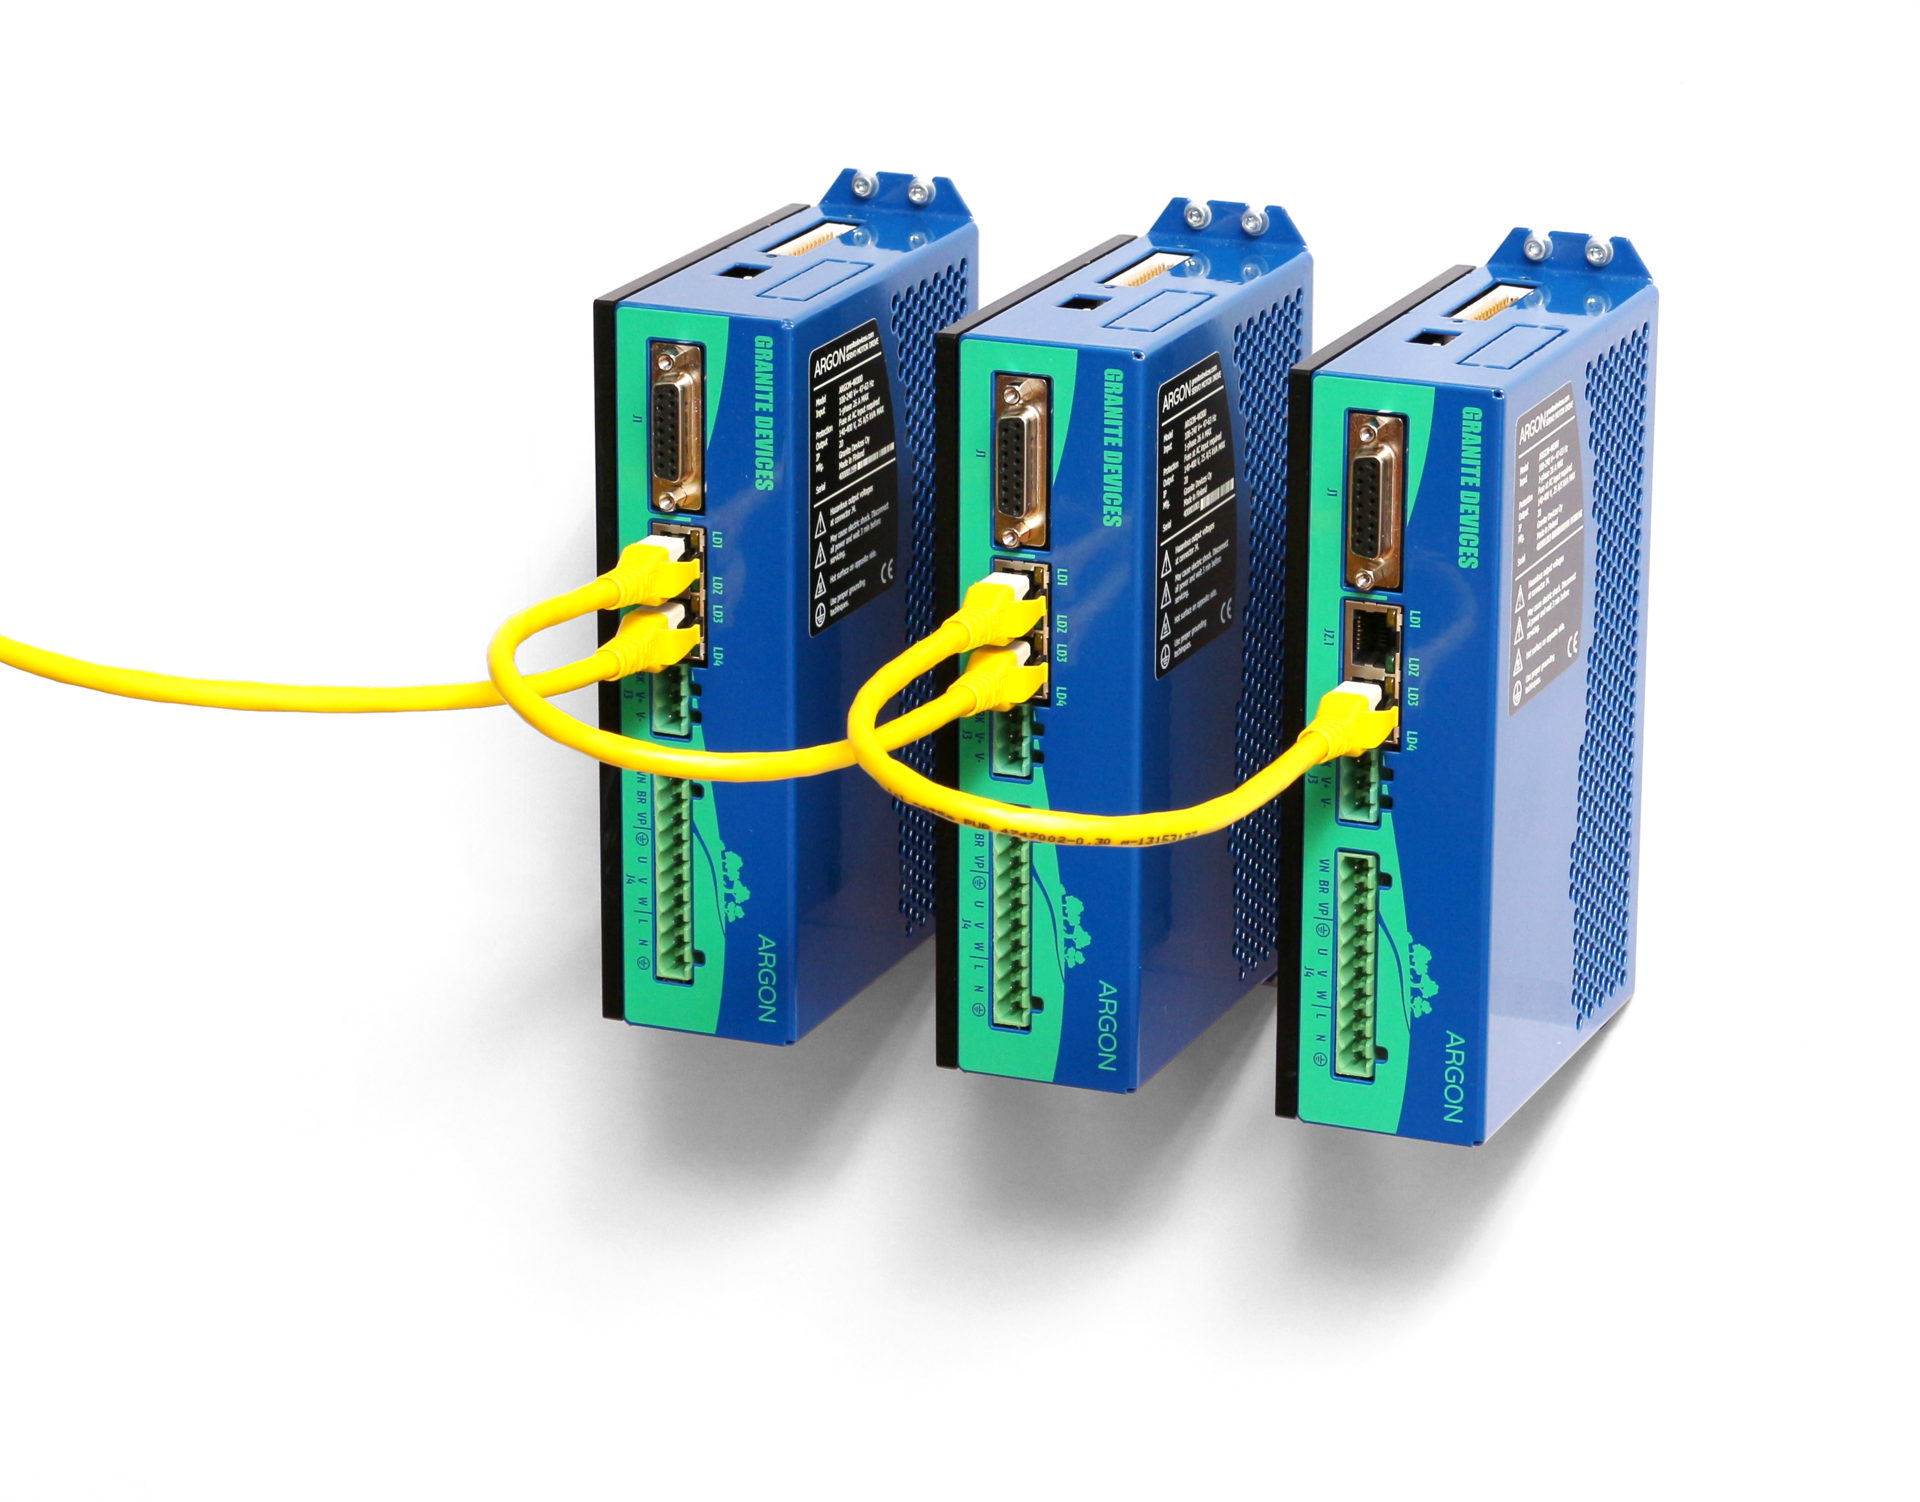
\includegraphics[width=.8\linewidth,height=2.3cm,keepaspectratio]{../figures/d4_servo_drives.png}\\
\credit{Tero Kontkanen, CC BY-SA 3.0, via Wikimedia Commons}
\end{columns}
\end{frame}

% ---------------------------------------------------------------------
\begin{frame}[t]{Clarke and Park transforms (amplitude-invariant form)}
\begin{columns}[T,onlytextwidth]
\column{.52\textwidth}
\begin{defbox}[Clarke: $abc\to\alpha\beta$ (stationary)]
\vspace{-2mm}
\[\begin{bmatrix} i_\alpha\\ i_\beta\end{bmatrix}=\frac23\begin{bmatrix}1&-\tfrac12&-\tfrac12\\[1pt] 0&\tfrac{\sqrt3}{2}&-\tfrac{\sqrt3}{2}\end{bmatrix}\begin{bmatrix} i_a\\ i_b\\ i_c\end{bmatrix}\]
With $i_a+i_b+i_c=0$: \ $i_\alpha=i_a$,\ \ $i_\beta=(i_a+2i_b)/\sqrt3$ -- only two sensors needed.
\end{defbox}
\begin{defbox}[Park: $\alpha\beta\to dq$ (rotating with $\theta_e$)]
\vspace{-2mm}
\[\begin{bmatrix} i_d\\ i_q\end{bmatrix}=\begin{bmatrix}\cos\theta_e&\sin\theta_e\\ -\sin\theta_e&\cos\theta_e\end{bmatrix}\begin{bmatrix} i_\alpha\\ i_\beta\end{bmatrix}\]
\vspace{-3mm}
\end{defbox}
\column{.46\textwidth}
\begin{itemize}\small
\item Factor $\tfrac23$: \hl{amplitude-invariant} -- a balanced set of peak $\hat I$ gives $|\vec i|=\hat I$.
\item Price: power is not invariant:
\end{itemize}
\begin{eqbox}\small\centering
$p=\tfrac32\left(v_\alpha i_\alpha+v_\beta i_\beta\right)=\tfrac32\left(v_d i_d+v_q i_q\right)$
\end{eqbox}
\begin{itemize}\small
\item Power-invariant variant uses $\sqrt{2/3}$ instead of $\tfrac23$ (no $\tfrac32$ in $p$ and $T$) -- check which one a drive manual uses!
\item Inverse Park ($dq\to\alpha\beta$) uses the transposed rotation; inverse Clarke: $i_a=i_\alpha$, $i_{b,c}=-\tfrac12i_\alpha\pm\tfrac{\sqrt3}2i_\beta$.
\item Zero-sequence $i_0=\tfrac13(i_a+i_b+i_c)=0$ for a star without neutral.
\end{itemize}
\src{[Park, 1929]; [Clarke, 1943]}
\end{columns}
\end{frame}

% ---------------------------------------------------------------------
\begin{frame}[t]{Reference frames: $abc$, $\alpha\beta$ and $dq$}
\begin{columns}[T,onlytextwidth]
\column{.48\textwidth}
\centering
\begin{tikzpicture}[scale=1.9]
  \def\th{60}\def\ga{40}\def\I{1.15}
  \foreach \a/\n in {0/a,120/b,240/c}{\draw[mkGray!70,dashed] (0,0) -- (\a:1.3); \node[font=\scriptsize,mkGray] at (\a:1.42) {$\n$};}
  \draw[-{Latex[length=1.8mm]},mkMid,line width=.7pt] (0,0) -- (1.55,0) node[right,font=\scriptsize]{$\alpha$};
  \draw[-{Latex[length=1.8mm]},mkMid,line width=.7pt] (0,0) -- (0,1.45) node[above,font=\scriptsize]{$\beta$};
  \draw[-{Latex[length=1.8mm]},mkBlue,line width=1pt] (0,0) -- (\th:1.5) node[above right,font=\scriptsize,inner sep=1pt]{$d$};
  \draw[-{Latex[length=1.8mm]},mkBlue,line width=1pt] (0,0) -- (\th+90:1.45) node[left,font=\scriptsize,inner sep=2pt]{$q$};
  \draw[mkBlue] (.42,0) arc (0:\th:.42); \node[font=\scriptsize,mkBlue] at (28:.56) {$\theta_e$};
  \draw[-{Latex[length=2mm]},mkOrange,line width=1.3pt] (0,0) -- (\th+\ga:\I) node[above,font=\scriptsize]{$\vec i_s$};
  \draw[mkOrange,densely dotted] (\th+\ga:\I) -- (\th:{\I*cos(\ga)}) node[right,font=\tiny]{$i_d$};
  \draw[mkOrange,densely dotted] (\th+\ga:\I) -- (\th+90:{\I*sin(\ga)}) node[below left,font=\tiny,inner sep=1pt]{$i_q$};
  \draw[mkMid,densely dotted] (\th+\ga:\I) -- (0,{\I*sin(\th+\ga)}) node[left,font=\tiny]{$i_\beta$};
  \draw[mkMid,densely dotted] (\th+\ga:\I) -- ({\I*cos(\th+\ga)},0) node[below,font=\tiny]{$i_\alpha$};
  \draw[mkGray,-{Latex[length=1.5mm]}] (20:1.2) arc (20:40:1.2); \node[font=\tiny,mkGray] at (30:1.33) {$\omega_e$};
\end{tikzpicture}
\column{.50\textwidth}
\begin{itemize}\small
\item \term{$abc$}: physical phase axes, $120^\circ$ apart (windings).
\item \term{$\alpha\beta$}: orthogonal, stationary; $\alpha\equiv a$. Quantities rotate at $\omega_e$.
\item \term{$dq$}: orthogonal, rotates with the rotor, $d$ on the magnet north pole: $\theta_e=\int\omega_e\,dt$.
\item The current \emph{vector} is the same physical object in all three frames -- only the coordinates change.
\item Space-vector notation:
\[\vec i_s^{\,dq}= \vec i_s^{\,\alpha\beta}\,e^{-j\theta_e},\qquad \vec i_s^{\,\alpha\beta}=\tfrac23\left(i_a+\underline a\,i_b+\underline a^2i_c\right)\]
\end{itemize}
\end{columns}
\end{frame}

% ---------------------------------------------------------------------
\begin{frame}[t]{The same current seen in the three frames}
\begin{columns}[T,onlytextwidth]
\column{.62\textwidth}
\begin{tikzpicture}
\begin{groupplot}[group style={group size=1 by 3,vertical sep=3mm,xticklabels at=edge bottom},
  mkplot,width=7.9cm,height=2.55cm,xmin=0,xmax=720,xtick={0,180,...,720},ymin=-12.5,ymax=12.5,ytick={-10,0,10},
  legend style={at={(1.01,.5)},anchor=west},grid=major]
\nextgroupplot[ylabel={$abc$ (A)}]
\addplot[mkBlue,thick,domain=0:720,samples=160] {(x<360?5:10)*cos(x+90)};
\addplot[mkOrange,thick,domain=0:720,samples=160] {(x<360?5:10)*cos(x+90-120)};
\addplot[mkSky,thick,domain=0:720,samples=160] {(x<360?5:10)*cos(x+90+120)};
\legend{$i_a$,$i_b$,$i_c$}
\nextgroupplot[ylabel={$\alpha\beta$ (A)}]
\addplot[mkBlue,thick,domain=0:720,samples=160] {-(x<360?5:10)*sin(x)};
\addplot[mkOrange,thick,domain=0:720,samples=160] {(x<360?5:10)*cos(x)};
\legend{$i_\alpha$,$i_\beta$}
\nextgroupplot[ylabel={$dq$ (A)},xlabel={$\theta_e$ (deg)}]
\addplot[mkBlue,thick,domain=0:720,samples=3] {0};
\addplot[mkOrange,thick,const plot] coordinates {(0,5) (360,10) (720,10)};
\legend{$i_d$,$i_q$}
\end{groupplot}
\end{tikzpicture}
\column{.36\textwidth}
\begin{itemize}\small
\item Balanced currents $i_a=\hat I\cos(\theta_e+90^\circ)$ etc.\ with a step $\hat I: 5\to\SI{10}{A}$ at $\theta_e=360^\circ$.
\item $\alpha\beta$: still sinusoidal, frequency $\omega_e$.
\item $dq$: \hl{DC}: $i_d=0$, $i_q=\hat I$ -- the step is a clean step.
\item A PI controller in $dq$ therefore tracks a sinusoid without phase lag at any speed (it is an \emph{integrator at} $\omega_e$ in $\alpha\beta$).
\end{itemize}
\end{columns}
\end{frame}

% ---------------------------------------------------------------------
\begin{frame}[t]{Electrical vs.\ mechanical angle: $\theta_e = p\,\theta_m$}
\begin{columns}[T,onlytextwidth]
\column{.55\textwidth}
\begin{tikzpicture}
\begin{axis}[mkplot,width=8.0cm,height=4.2cm,xmin=0,xmax=360,ymin=0,ymax=370,xtick={0,90,...,360},ytick={0,180,360},
  xlabel={mechanical angle $\theta_m$ (deg)},ylabel={$\theta_e \bmod 360^\circ$},legend pos=north west]
\addplot[mkOrange,thick] coordinates {(0,0) (90,360) (90,0) (180,360) (180,0) (270,360) (270,0) (360,360)};
\addplot[mkBlue,thick,dashed] coordinates {(0,0) (360,360)};
\legend{$\theta_e$ ($p=4$),$\theta_m$}
\end{axis}
\end{tikzpicture}
\begin{eqbox}\small\centering
$\theta_e=p\,\theta_m,\quad \omega_e=p\,\omega_m,\quad f_e=\dfrac{p\,n}{60}$
\end{eqbox}
\scriptsize Example: $p=4$, $n=\SI{3000}{rpm}$ $\Rightarrow$ $f_e=\SI{200}{Hz}$, $\omega_e=\SI{1257}{rad/s}$.
\column{.43\textwidth}
\centering
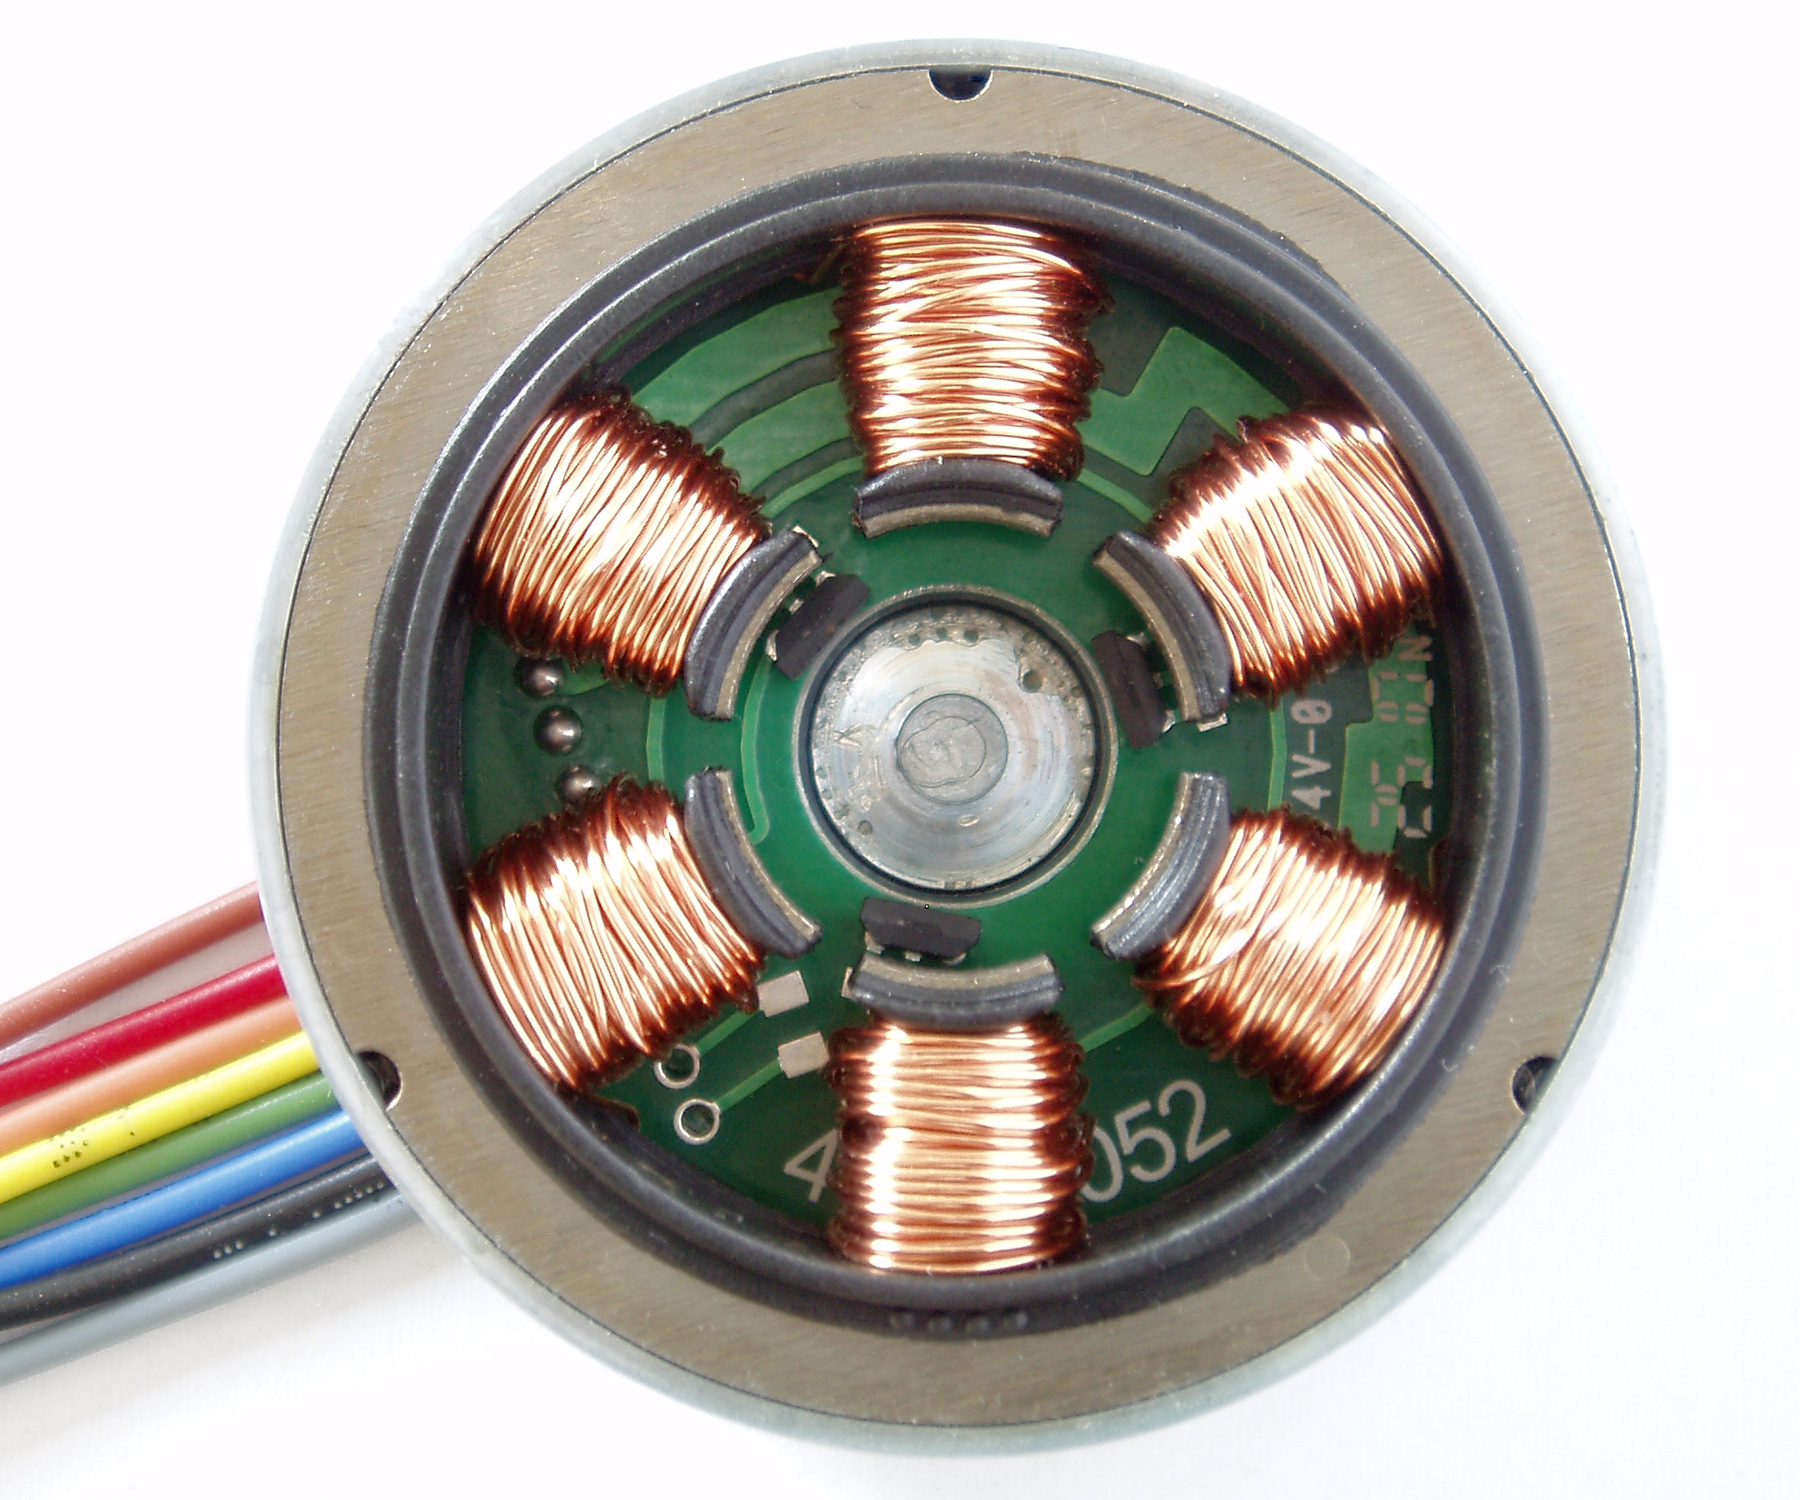
\includegraphics[width=.5\linewidth]{../figures/d4_bldc_stator.jpg}\\
\credit{12-slot stator. Medvedev, CC BY-SA 3.0, via Wikimedia Commons}
\begin{itemize}\scriptsize
\item $p$ = number of \emph{pole pairs} (an 8-pole motor has $p=4$).
\item Encoder resolution in electrical degrees is $p$ times coarser.
\item A mechanical alignment error $\Delta\theta_m$ becomes $p\,\Delta\theta_m$ in the Park transform.
\end{itemize}
\end{columns}
\end{frame}

% ---------------------------------------------------------------------
\begin{frame}[t]{PMSM model in rotor ($dq$) coordinates}
\begin{columns}[T,onlytextwidth]
\column{.50\textwidth}
\small Stator equation in stationary coordinates (space vectors):
\[\vec v_s=R\,\vec i_s+\frac{d\vec\psi_s}{dt}\]
Substitute $\vec x=\vec x^{\,dq}e^{j\theta_e}$:
\[\vec v^{\,dq}=R\,\vec i^{\,dq}+\frac{d\vec\psi^{\,dq}}{dt}+j\omega_e\vec\psi^{\,dq}\]
Flux linkages (rotor frame, no saturation):
\[\psi_d=L_di_d+\psi_\text{PM},\qquad \psi_q=L_qi_q\]
\column{.48\textwidth}
\begin{eqbox}\small
\vspace{-3mm}
\begin{align*}
v_d&=R\,i_d+L_d\frac{di_d}{dt}\underbrace{-\,\omega_eL_qi_q}_{\text{cross-coupling}}\\
v_q&=R\,i_q+L_q\frac{di_q}{dt}\underbrace{+\,\omega_eL_di_d}_{\text{cross-coupling}}\underbrace{+\,\omega_e\psi_\text{PM}}_{\text{back-EMF}}
\end{align*}
\vspace{-4mm}
\end{eqbox}
\begin{itemize}\scriptsize
\item Units: V, A, H, Vs; $\omega_e$ in rad/s (electrical). Motor sign convention (power into terminals positive).
\item The rotational term $j\omega_e\vec\psi$ produces the \hl{speed-dependent coupling} between axes and the back-EMF on the $q$-axis only.
\item SPM: $L_d\approx L_q=L$; IPM: $L_q>L_d$ (saliency).
\item Mechanics: $J\dot\omega_m=T_e-B\omega_m-T_L$.
\end{itemize}
\end{columns}
\end{frame}

% ---------------------------------------------------------------------
\begin{frame}[t]{Equivalent circuits of the $d$- and $q$-axis}
\centering
\begin{circuitikz}[scale=.76,transform shape,line width=.5pt]
  % d-axis
  \node[font=\small\bfseries,mkBlue] at (2.5,3.0) {$d$-axis};
  \draw (0,0) to[short,o-] (0,2.2) to[R,l=$R$] (2.2,2.2) to[L,l=$L_d$,i>^=$i_d$] (4.6,2.2) -- (5.2,2.2)
        to[cV,l=$\omega_eL_qi_q$] (5.2,0) -- (0,0) node[ocirc]{};
  \draw[-{Latex[length=2mm]}] (-.5,.2) -- node[left]{$v_d$} (-.5,2.0);
  \node[font=\footnotesize,mkRed] at (4.75,1.65) {$-$}; \node[font=\footnotesize,mkRed] at (4.75,.55) {$+$};
  % q-axis
  \begin{scope}[xshift=8.8cm]
  \node[font=\small\bfseries,mkOrange] at (3.5,3.0) {$q$-axis};
  \draw (0,0) to[short,o-] (0,2.2) to[R,l=$R$] (2.2,2.2) to[L,l=$L_q$,i>^=$i_q$] (4.6,2.2)
        to[cV,l=$\omega_eL_di_d$] (7.0,2.2) to[V,l=$\omega_e\psi_\text{PM}$] (7.0,0) -- (0,0) node[ocirc]{};
  \draw[-{Latex[length=2mm]}] (-.5,.2) -- node[left]{$v_q$} (-.5,2.0);
  \node[font=\footnotesize,mkRed] at (5.05,1.75) {$+$}; \node[font=\footnotesize,mkRed] at (6.55,1.75) {$-$};
  \node[font=\footnotesize,mkRed] at (7.45,.45) {$-$}; \node[font=\footnotesize,mkRed] at (7.45,1.75) {$+$};
  \end{scope}
\end{circuitikz}\\[-1mm]
{\scriptsize\color{mkGray} red signs: polarity of each speed voltage as a voltage drop in the direction of the current}
\vspace{1mm}
\begin{columns}[T,onlytextwidth]
\column{.48\textwidth}
\begin{itemize}\small
\item Each axis is an \term{$R$--$L$ circuit} with a speed-dependent voltage source.
\item Electrical time constants $\tau_d=L_d/R$, $\tau_q=L_q/R$ (here \SI{6}{ms}).
\end{itemize}
\column{.50\textwidth}
\begin{itemize}\small
\item The sources are \hl{disturbances} for the current loops: known (measured $i$, $\omega_e$) $\Rightarrow$ can be fed forward (decoupling).
\item $q$-axis carries the back-EMF; it sets the voltage requirement at speed.
\end{itemize}
\end{columns}
\end{frame}

% ---------------------------------------------------------------------
\begin{frame}[t]{Torque: flux- and torque-producing currents, reluctance torque}
\begin{columns}[T,onlytextwidth]
\column{.48\textwidth}
\begin{eqbox}\small
\vspace{-3mm}
\begin{align*}
T_e&=\tfrac32\,p\,(\psi_d i_q-\psi_q i_d)\\
&=\tfrac32\,p\,\big[\underbrace{\psi_\text{PM}\,i_q}_{\text{magnet}}+\underbrace{(L_d-L_q)\,i_d i_q}_{\text{reluctance}}\big]
\end{align*}
\vspace{-4mm}
\end{eqbox}
\begin{itemize}\scriptsize
\item SPM ($L_d=L_q$): $T_e=k_t i_q$, $k_t=\tfrac32p\psi_\text{PM}$ \\(\SI{0.72}{Nm/A} for the reference motor); $i_d^*=0$ minimises $|\vec i|$.
\item IPM ($L_q>L_d$): \hl{negative $i_d$ adds torque}.
\item With $i_d=-\hat I\sin\beta$, $i_q=\hat I\cos\beta$:\\
$T_e=\tfrac32p\left[\psi_\text{PM}\hat I\cos\beta+\tfrac12(L_q-L_d)\hat I^2\sin2\beta\right]$
\item Note: $k_t$ in Nm/A refers to the \emph{peak} (amplitude-invariant) current; datasheets often use rms: $k_{t,\text{rms}}=\sqrt2\,k_t$.
\end{itemize}
\column{.50\textwidth}
\begin{tikzpicture}
\begin{axis}[mkplot,width=7.4cm,height=5.4cm,xmin=0,xmax=90,ymin=-.5,ymax=14,xtick={0,15,...,90},
  xlabel={current angle $\beta$ from $q$-axis (deg)},ylabel={torque (Nm)},legend pos=south west]
\addplot[mkBlue,thick,domain=0:90,samples=91] {9.6*cos(x)};
\addplot[mkSky,thick,dashed,domain=0:90,samples=91] {3.6*sin(2*x)};
\addplot[mkOrange,line width=1.2pt,domain=0:90,samples=91] {9.6*cos(x)+3.6*sin(2*x)};
\addplot[only marks,mark=*,mark size=1.5pt,mkRed] coordinates {(26.6,11.47)};
\node[font=\tiny,mkRed,anchor=south west] at (axis cs:20,11.9) {MTPA: $\beta=26.6^\circ$, \SI{11.5}{Nm}};
\legend{magnet,reluctance,total}
\end{axis}
\end{tikzpicture}\\
\scriptsize Illustrative IPM: $p=4$, $\psi_\text{PM}=\SI{0.08}{Vs}$, $L_d=\SI{2}{mH}$, $L_q=\SI{5}{mH}$, $\hat I=\SI{20}{A}$ (+19\,\% vs.\ $i_d=0$).
\end{columns}
\end{frame}

% ---------------------------------------------------------------------
\begin{frame}[t]{Maximum torque per ampere (MTPA)}
\begin{columns}[T,onlytextwidth]
\column{.50\textwidth}
\centering
\begin{tikzpicture}
\begin{axis}[mkplot,width=7.0cm,height=5.8cm,axis equal image,xmin=-25,xmax=2,ymin=0,ymax=31,
  xlabel={$i_d$ (A)},ylabel={$i_q$ (A)},legend pos=north west,legend style={font=\tiny}]
\addplot[mkGray,densely dotted,domain=90:180,samples=40] ({10*cos(x)},{10*sin(x)});
\addplot[mkGray,densely dotted,domain=90:180,samples=40,forget plot] ({20*cos(x)},{20*sin(x)});
\addplot[mkSky,thick,domain=-25:0,samples=60] {4/(6*(0.08-0.003*x))};
\addplot[mkMid,thick,domain=-25:0,samples=60] {8/(6*(0.08-0.003*x))};
\addplot[mkBlue,thick,domain=-25:0,samples=60] {12/(6*(0.08-0.003*x))};
\addplot[mkOrange,line width=1.3pt,domain=0:25,samples=60] ({6.667-sqrt(44.44+x^2/2)},{sqrt(max(x^2-(6.667-sqrt(44.44+x^2/2))^2,0))});
\legend{{$\lvert\vec i\rvert=10$; $20$\,A},\SI{4}{Nm},\SI{8}{Nm},\SI{12}{Nm},MTPA}
\end{axis}
\end{tikzpicture}
\column{.48\textwidth}
\begin{itemize}\small
\item Goal: minimum $|\vec i|$ (copper loss, inverter current) for a required torque.
\item Condition: constant-torque curve \hl{tangent} to the current circle. Setting $\partial T_e/\partial\beta=0$:
\end{itemize}
\begin{eqbox}\small
\[i_d^\text{MTPA}=\frac{\psi_\text{PM}}{4(L_q-L_d)}-\sqrt{\frac{\psi_\text{PM}^2}{16(L_q-L_d)^2}+\frac{\hat I^2}{2}}\]
\vspace{-5mm}
\end{eqbox}
\begin{itemize}\scriptsize
\item SPM: $L_q=L_d$ $\Rightarrow$ MTPA is simply $i_d=0$.
\item Implementation: look-up table $i_d^*=f(i_q^*)$ or $(i_d^*,i_q^*)=f(T^*)$; tables measured on a dynamometer include saturation ($L_q$ drops with $i_q$).
\end{itemize}
\src{[Jahns, Kliman \& Neumann, 1986]}
\end{columns}
\end{frame}

% ---------------------------------------------------------------------
\begin{frame}[t]{Field weakening (brief) and the torque--speed envelope}
\begin{columns}[T,onlytextwidth]
\column{.52\textwidth}
\begin{tikzpicture}
\begin{axis}[mkplot,width=7.0cm,height=5.0cm,xmin=0,xmax=8000,ymin=0,ymax=16,
  xlabel={speed $n$ (rpm)},ylabel={torque (Nm)},legend pos=north east,
  scaled x ticks=false,xticklabel style={/pgf/number format/fixed},axis y line*=left]
\addplot[mkBlue,line width=1.1pt] table[x=rpm,y=T]{data/fw.dat};
\addplot[mkRed,thick,dashed] coordinates {(3240,0) (3240,16)};
\legend{max.\ torque}
\end{axis}
\begin{axis}[mkplot,width=7.0cm,height=5.0cm,xmin=0,xmax=8000,ymin=-22,ymax=6,axis y line*=right,axis x line=none,
  ylabel={$i_d$ (A), $P$ (kW)},legend pos=south west,grid=none]
\addplot[mkOrange,thick] table[x=rpm,y=id]{data/fw.dat};
\addplot[mkMid,thick,dotted] table[x=rpm,y=P]{data/fw.dat};
\legend{$i_d$,$P$}
\end{axis}
\end{tikzpicture}\\
\scriptsize Computed for the reference SPM ($V_\text{dc}=\SI{325}{V}$, $\hat I_\text{max}=\SI{20}{A}$): base speed $\approx$\,\SI{3240}{rpm}, limit $\approx$\,\SI{7440}{rpm}.
\column{.46\textwidth}
\begin{itemize}\small
\item Above base speed the back-EMF $\omega_e\psi_\text{PM}$ approaches $V_\text{max}$.
\item Negative $i_d$ \hl{reduces the $d$-axis flux} $L_di_d+\psi_\text{PM}$ $\Rightarrow$ more speed at the same voltage.
\item The current budget used by $i_d$ is lost for $i_q$: torque falls, power roughly constant.
\item Characteristic current $I_\text{ch}=\psi_\text{PM}/L_d$ (here \SI{40}{A} $>\hat I_\text{max}$ $\Rightarrow$ finite maximum speed).
\item Practical: voltage-feedback FW loop ($|\vec v^*|>0.95V_\text{max}\Rightarrow$ integrate towards negative $i_d^*$).
\item Servo motors seldom use deep FW; spindles and traction do.
\end{itemize}
\end{columns}
\end{frame}

% ---------------------------------------------------------------------
\begin{frame}[t]{Worked example: steady-state operating point at \SI{3000}{rpm}}
\begin{columns}[T,onlytextwidth]
\column{.50\textwidth}
\footnotesize
Reference SPM, $i_d=0$, $i_q=\SI{10}{A}$, $n=\SI{3000}{rpm}$:
\begin{align*}
\omega_e&=p\,\tfrac{2\pi n}{60}=4\cdot314.2=\SI{1256.6}{rad/s}\\
E&=\omega_e\psi_\text{PM}=\SI{150.8}{V}\\
v_q&=R\,i_q+E=5.0+150.8=\SI{155.8}{V}\\
v_d&=-\omega_eL\,i_q=\SI{-37.7}{V}\\
|\vec v|&=\sqrt{v_d^2+v_q^2}=\SI{160.3}{V}\ (85\,\%\text{ of }V_\text{max}=\SI{187.6}{V})\\
T_e&=k_ti_q=\SI{7.2}{Nm},\quad P_\text{mech}=T_e\omega_m=\SI{2.26}{kW}\\
P_\text{el}&=\tfrac32(v_di_d+v_qi_q)=\SI{2.34}{kW}
\end{align*}
Check: $P_\text{el}-P_\text{mech}=\tfrac32R\,i_q^2=\SI{75}{W}$ \textcolor{mkGreen}{\checkmark}
\column{.48\textwidth}
\centering
\begin{tikzpicture}[scale=1]
  \draw[-{Latex[length=2mm]},mkGray] (-1.3,0) -- (1.5,0) node[right,font=\scriptsize]{$d$};
  \draw[-{Latex[length=2mm]},mkGray] (0,-.2) -- (0,4.0) node[above,font=\scriptsize]{$q$};
  % scale: 40 V per cm
  \draw[-{Latex[length=2mm]},mkOrange,line width=1.4pt] (0,0) -- (0,1.6) node[midway,right,font=\scriptsize]{$\vec i\,(i_q)$};
  \draw[-{Latex[length=2mm]},mkMid,line width=1pt] (0,0) -- (0,3.77) node[pos=.62,right,font=\scriptsize]{$E=\omega_e\psi_\text{PM}$};
  \draw[-{Latex[length=2mm]},mkSky,line width=1pt] (0,3.77) -- (0,3.895);
  \node[font=\tiny,mkSky,anchor=west] at (.05,3.95) {$Ri_q$};
  \draw[-{Latex[length=2mm]},mkRed,line width=1pt] (0,3.895) -- (-.943,3.895) node[midway,above,font=\scriptsize]{$-\omega_eLi_q$};
  \draw[-{Latex[length=2mm]},mkBlue,line width=1.4pt] (0,0) -- (-.943,3.895) node[left,font=\scriptsize,pos=.55]{$\vec v$};
  \draw[mkBlue] (0,1.0) arc (90:103.6:1.0); \node[font=\tiny,mkBlue] at (-.32,1.25) {$\varphi$};
  \draw[-{Latex[length=2mm]},mkGray,line width=.8pt] (0,0) -- (1.2,0) node[below,font=\tiny]{$\psi_\text{PM}$};
\end{tikzpicture}\\
\scriptsize Vector diagram to scale (voltages \SI{40}{V/cm}); $\varphi=13.6^\circ$, $\cos\varphi=0.97$.
The $\omega_eLi_q$ term grows with load and speed -- it consumes voltage reserve.
\end{columns}
\end{frame}

% ---------------------------------------------------------------------
\begin{frame}[t]{FOC: the basic structure}
\centering
\begin{tikzpicture}[x=.92cm,y=.85cm]
  % forward path
  \node[sumn] (sw) at (0.5,2.4) {};
  \node[blk,minimum width=10mm] (pw) at (1.6,2.4) {PI $\omega$};
  \node[sumn] (sq) at (3.3,2.4) {};
  \node[blk,minimum width=10mm] (pq) at (4.4,2.4) {PI $i_q$};
  \node[sumn] (sd) at (2.9,1.0) {};
  \node[blk,minimum width=10mm] (pd) at (4.4,1.0) {PI $i_d$};
  \node[blko,minimum height=22mm,minimum width=12mm] (dec) at (6.0,1.7) {decou-\\pling\\+ FF};
  \node[blk,minimum height=22mm,minimum width=12mm] (ipark) at (7.7,1.7) {inverse\\Park\\$dq\!\to\!\alpha\beta$};
  \node[blk,minimum height=22mm,minimum width=12mm] (svm) at (9.3,1.7) {SVPWM};
  \node[blko,minimum height=22mm,minimum width=12mm] (inv) at (10.9,1.7) {VSI\\inverter};
  \node[draw=mkBlue,circle,minimum size=11mm,fill=mkPale,font=\scriptsize,line width=.6pt] (m) at (12.9,1.7) {PMSM};
  \node[blk,minimum width=8mm] (enc) at (14.3,1.7) {enc.};
  \draw[mkBlue,line width=1pt] (m.east) -- (enc.west);
  % feedback blocks
  \node[blk,minimum width=14mm] (park) at (6.6,-0.55) {Clarke + Park};
  \node[blk,minimum width=12mm] (pp) at (11.0,-1.2) {$\times p,\ +\theta_\text{off}$};
  \node[blk,minimum width=12mm] (dd) at (12.9,-2.0) {$d/dt$ + filter};
  % forward signals
  \draw[sig] (-.4,2.4) node[left,font=\scriptsize]{$\omega^*$} -- (sw);
  \draw[sig] (sw) -- (pw); \draw[sig] (pw) -- node[above,lab]{$i_q^*$} (sq);
  \draw[sig] (sq) -- (pq); \draw[sig] (sd) -- (pd);
  \draw[sig] (1.7,1.0) node[left,font=\scriptsize,align=right]{$i_d^*$ (0/MTPA/FW)} -- (sd);
  \draw[sig] (pq.east) -- (pq.east -| dec.west); \draw[sig] (pd.east) -- (pd.east -| dec.west);
  \draw[sig] (dec.east |- 0,2.4) -- node[above,lab]{$v_q^*$} (ipark.west |- 0,2.4);
  \draw[sig] (dec.east |- 0,1.0) -- node[below,lab]{$v_d^*$} (ipark.west |- 0,1.0);
  \draw[sig] (ipark.east |- 0,2.4) -- node[above,lab]{$v_\alpha^*$} (svm.west |- 0,2.4);
  \draw[sig] (ipark.east |- 0,1.0) -- node[below,lab]{$v_\beta^*$} (svm.west |- 0,1.0);
  \foreach \y in {1.4,1.7,2.0}{\draw[sig] (svm.east |- 0,\y) -- (inv.west |- 0,\y);}
  \node[lab,above] at (10.1,2.45) {gates};
  \foreach \y in {1.45,1.7,1.95}{\draw[mkNavy,line width=.8pt] (inv.east |- 0,\y) -- (m.west |- 0,\y);}
  \draw[mkGray,-{Latex[length=1.5mm]}] (10.9,3.25) node[above,font=\tiny]{$V_\text{dc}$} -- (inv.north);
  % current feedback
  \fill[mkOrange] (11.85,1.45) circle (1.3pt); \fill[mkOrange] (12.05,1.7) circle (1.3pt);
  \draw[fb] (11.85,1.45) -- (11.85,-0.4) -- (park.east |- 0,-0.4);
  \draw[fb] (12.05,1.7) -- (12.05,-0.7) -- node[below,lab,pos=.7]{$i_a,\,i_b$} (park.east |- 0,-0.7);
  \draw[fb] (park.west |- 0,-0.4) -- node[above,lab,pos=.15]{$i_d$} (2.9,-0.4) -- (sd.south);
  \draw[fb] (park.west |- 0,-0.7) -- node[below,lab,pos=.15]{$i_q$} (3.3,-0.7) -- (sq.south);
  % angle path
  \draw[fb] (enc.south) |- (pp.east);
  \draw[fb] (pp.west) -- node[above,lab,pos=.3]{$\theta_e$} (8.0,-1.2) -- (8.0,0.6);
  \draw[fb] (8.0,-1.2) -- (6.6,-1.2) -- (park.south);
  \draw[fb] (14.3,-1.2) |- (dd.east);
  \draw[fb] (dd.west) -- (0.5,-2.0) node[pos=.95,above,lab]{$\omega_m$} -- (sw.south);
  \draw[ff] (5.3,-2.0) -- node[pos=.12,right,lab]{$\omega_e$} (5.3,0.6);
  \node[font=\tiny,mkGray] at (.3,2.05) {$-$}; \node[font=\tiny,mkGray] at (3.5,2.05) {$-$}; \node[font=\tiny,mkGray] at (3.1,.65) {$-$};
\end{tikzpicture}
\vspace{1mm}
\begin{columns}[T,onlytextwidth]
\column{.5\textwidth}
\scriptsize \textbf{Every PWM period:} sample $i_a,i_b$ and $\theta_m$ $\to$ Clarke/Park $\to$ two PIs $\to$ decoupling $\to$ inverse Park $\to$ SVPWM duty update.
\column{.48\textwidth}
\scriptsize Velocity loop: every 1--4 PWM periods. The outer position loop (Session 3.4) provides $\omega^*$. Typical current-loop execution: 5--20\,\si{\micro s} on a DSP/MCU.
\end{columns}
\end{frame}

% ---------------------------------------------------------------------
\begin{frame}[t]{Cross-coupling and decoupling}
\begin{columns}[T,onlytextwidth]
\column{.42\textwidth}
\begin{itemize}\small
\item Without compensation the $q$-loop must \emph{integrate up} the back-EMF and both PIs fight the coupling terms $\omega_eL\,i$.
\item \term{Decoupling / feedforward}: add the model terms to the PI outputs:
\end{itemize}
\begin{eqbox}\small
\vspace{-3mm}
\begin{align*}
v_d^*&=v_{d,\text{PI}}-\omega_e\hat L_q\,i_q\\
v_q^*&=v_{q,\text{PI}}+\omega_e(\hat L_d\,i_d+\hat\psi_\text{PM})
\end{align*}
\vspace{-4mm}
\end{eqbox}
\begin{itemize}\scriptsize
\item Ideal decoupling leaves two independent $1/(R+Ls)$ plants.
\item Parameter errors and the loop delay leave a residual coupling (right: $i_d$ peak \SI{2.3}{A} $\to$ \SI{0.85}{A}).
\item Use $i^*$ instead of $i$ to avoid feeding noise.
\end{itemize}
\column{.56\textwidth}
\begin{tikzpicture}
\begin{groupplot}[group style={group size=1 by 2,vertical sep=3mm,xticklabels at=edge bottom},
  mkplot,width=8.2cm,height=3.3cm,xmin=0,xmax=1.5,legend pos=south east]
\nextgroupplot[ylabel={$i_q$ (A)},ymin=-1,ymax=12]
\addplot[mkSky,thick,dashed] table[x=t,y=iq_n]{data/decoup.dat};
\addplot[mkBlue,thick] table[x=t,y=iq_d]{data/decoup.dat};
\legend{PI only,PI + decoupling}
\nextgroupplot[ylabel={$i_d$ (A)},xlabel={time (ms)},ymin=-.6,ymax=2.6]
\addplot[mkOrange!80,thick,dashed] table[x=t,y=id_n]{data/decoup.dat};
\addplot[mkOrange,thick] table[x=t,y=id_d]{data/decoup.dat};
\end{groupplot}
\end{tikzpicture}\\
\scriptsize Simulated $i_q^*$ step $0\to\SI{10}{A}$ at \SI{3000}{rpm} (reference motor, discrete PI, \SI{16}{kHz}, 1.5\,$T_s$ delay; integrator pre-loaded with $\omega_e\psi_\text{PM}$ in both cases).
\end{columns}
\end{frame}

% ---------------------------------------------------------------------
\begin{frame}[t]{Rotor angle alignment and offset errors}
\begin{columns}[T,onlytextwidth]
\column{.50\textwidth}
\begin{itemize}\small
\item The encoder zero is arbitrary; FOC needs $\theta_e=0$ on the magnet $d$-axis: $\theta_e=p(\theta_m-\theta_{m,0})$.
\item \textbf{Methods}
\begin{itemize}\scriptsize
\item DC alignment: inject a current vector along $\alpha$, rotor locks to $\theta_e=0$, store $\theta_{m,0}$ (needs free shaft, light load).
\item Back-EMF: spin the motor externally, compare phase-voltage zero crossings with encoder.
\item Hall sensors for start-up, refined at the first Hall edge.
\item Absolute encoder with factory-stored offset (typical for servo motors).
\item Standstill methods with high-frequency injection (saliency / saturation).
\end{itemize}
\end{itemize}
\column{.48\textwidth}
\begin{tikzpicture}
\begin{axis}[mkplot,width=7.0cm,height=4.4cm,xmin=0,xmax=90,ymin=-.05,ymax=1.05,xtick={0,15,...,90},
  xlabel={electrical offset error $\Delta\theta_e$ (deg)},ylabel={per unit of $|\vec i|$},legend pos=south west]
\addplot[mkBlue,thick,domain=0:90,samples=60] {cos(x)};
\addplot[mkOrange,thick,dashed,domain=0:90,samples=60] {sin(x)};
\legend{torque-producing $i_q$,unwanted $i_d$}
\end{axis}
\end{tikzpicture}
\begin{notebox}
$T_e=k_t|\vec i|\cos\Delta\theta_e$. $\Delta\theta_m=2^\circ$ mech.\ with $p=4$ $\Rightarrow$ $8^\circ$ el.: $-1\,\%$ torque, but $14\,\%$ of the current in $d$ (heating, FW in one direction only). For $|\Delta\theta_e|>90^\circ$ torque reverses $\Rightarrow$ \hl{runaway}.
\end{notebox}
\end{columns}
\end{frame}

% ---------------------------------------------------------------------
\begin{frame}{Summary 3.3 -- Field-oriented control}
\begin{columns}[T,onlytextwidth]
\column{.58\textwidth}
\begin{keybox}[Key take-aways]
\small
\begin{itemize}
\item Clarke + Park map AC phase quantities into DC $dq$ quantities in the rotor frame; $\theta_e=p\,\theta_m$.
\item PMSM $dq$ model: two $R$--$L$ circuits + cross-coupling $\omega_eL\,i$ + back-EMF $\omega_e\psi_\text{PM}$.
\item $T_e=\tfrac32p[\psi_\text{PM}i_q+(L_d-L_q)i_di_q]$; SPM: $i_d^*=0$, IPM: MTPA with $i_d<0$.
\item Field weakening trades current for voltage above base speed.
\item FOC = angle + Park + 2 PI + decoupling + inverse Park + SVPWM, every PWM period.
\item Angle offset errors cost torque and can cause runaway.
\end{itemize}
\end{keybox}
\column{.38\textwidth}
\begin{notebox}
\textbf{Self-check}\\
1.\ $i_a=\SI{8}{A}$, $i_b=\SI{-4}{A}$: $i_\alpha$, $i_\beta$?\ ($8$; $0$)\\[1mm]
2.\ Why does $i_q$ step cleanly while $i_a$ is sinusoidal?\\[1mm]
3.\ Back-EMF of the reference motor at \SI{1500}{rpm}?\ (\SI{75.4}{V} peak phase)
\end{notebox}
\end{columns}
\end{frame}

% =====================================================================
\section{3.4 Current, Velocity and Position Loops}
% =====================================================================

\begin{frame}[t]{The nested (cascade) control structure}
\centering
\begin{tikzpicture}[x=.9cm,y=.9cm]
  \node[blko,minimum width=14mm] (tg) at (0,1.6) {trajectory\\generator};
  \node[sumn] (s1) at (1.6,1.6) {};
  \node[blk] (cp) at (2.7,1.6) {position\\P / PI};
  \node[sumn] (s2) at (4.1,1.6) {};
  \node[blk] (cv) at (5.2,1.6) {velocity\\PI};
  \node[sumn] (s3) at (6.6,1.6) {};
  \node[blk] (ci) at (7.7,1.6) {current\\PI (FOC)};
  \node[blko] (pwm) at (9.3,1.6) {PWM +\\inverter};
  \node[blk] (mot) at (10.9,1.6) {motor\\$k_t$};
  \node[blk] (mech) at (12.5,1.6) {mechanics\\$1/(Js)$};
  \node[blk,minimum width=8mm] (int) at (14.0,1.6) {$\tfrac1s$};
  \draw[sig] (tg) -- node[above,lab]{$x^*$} (s1); \draw[sig] (s1) -- (cp); \draw[sig] (cp) -- node[above,lab]{$\omega^*$} (s2);
  \draw[sig] (s2) -- (cv); \draw[sig] (cv) -- node[above,lab]{$i_q^*$} (s3); \draw[sig] (s3) -- (ci);
  \draw[sig] (ci) -- (pwm); \draw[sig] (pwm) -- (mot); \draw[sig] (mot) -- node[above,lab]{$T_e$} (mech);
  \draw[sig] (mech) -- node[above,lab]{$\omega$} (int); \draw[sig] (int) -- (14.8,1.6) node[right,font=\scriptsize]{$x$};
  \draw[sig] (12.5,2.6) node[above,font=\tiny]{$T_L$} -- (mech.north);
  % feedbacks
  \draw[fb] (10.4,1.15) -- (10.4,.7) -| (s3.south); \node[lab] at (8.9,.55) {$i$ (\SI{16}{kHz})};
  \draw[fb] (13.3,1.6) -- (13.3,.1) -| (s2.south); \node[lab] at (8.9,-.05) {$\omega$ (\SI{8}{kHz})};
  \draw[fb] (14.6,1.6) -- (14.6,-.5) -| (s1.south); \node[lab] at (8.9,-.65) {$x$ (\SI{2}{kHz})};
  % feedforward
  \draw[ff] (tg.north) |- (5.0,2.65) node[pos=.6,above,lab]{$\dot x^*$ velocity FF} -- (s2.north);
  \draw[ff] (tg.north) ++(.3,0) |- (6.6,3.1) node[pos=.75,above,lab]{$J\ddot x^*/k_t$ torque FF} -- (s3.north);
  \node[font=\tiny,mkGray] at (1.4,1.25) {$-$}; \node[font=\tiny,mkGray] at (3.9,1.25) {$-$}; \node[font=\tiny,mkGray] at (6.4,1.25) {$-$};
\end{tikzpicture}\\[2mm]
\begin{columns}[T,onlytextwidth]
\column{.5\textwidth}
\begin{itemize}\small
\item Each loop sees the closed inner loop as its ``actuator''.
\item Inner loops are faster, sampled faster, and \hl{limit} the variables of the outer loop (current $\to$ torque, velocity).
\end{itemize}
\column{.48\textwidth}
\begin{itemize}\small
\item Tuned and commissioned \emph{inside out}.
\item Feedforward paths (dashed) carry the known reference derivatives past the slow loops.
\end{itemize}
\end{columns}
\src{[Ellis, 2012]; [Lorenz, Lipo \& Novotny, 1994]}
\end{frame}

% ---------------------------------------------------------------------
\begin{frame}[t]{Interaction between loops: the bandwidth hierarchy}
\begin{columns}[T,onlytextwidth]
\column{.55\textwidth}
\begin{tikzpicture}[x=1.12cm,y=1cm]
  \draw[-{Latex[length=2mm]},mkGray] (0,0) -- (5.2,0) node[right,font=\scriptsize]{$f$ (Hz)};
  \foreach \e/\l in {0/1,1/10,2/100,3/1k,4/10k,5/100k}{\draw[mkGray] (\e,0) -- (\e,-.1) node[below,font=\tiny]{\l};}
  \fill[mkSky!60] (1.0,2.9) rectangle (1.9,3.4); \node[font=\scriptsize,anchor=east] at (.95,3.15) {position 10--80\,Hz};
  \fill[mkMid!70] (1.7,2.1) rectangle (2.6,2.6); \node[font=\scriptsize,anchor=east] at (1.65,2.35) {velocity 50--400\,Hz};
  \fill[mkBlue!80] (2.7,1.3) rectangle (3.5,1.8); \node[font=\scriptsize,anchor=west] at (3.55,1.55) {current 0.5--3\,kHz};
  \fill[mkOrange!80] (3.9,.5) rectangle (4.6,1.0); \node[font=\scriptsize,anchor=west] at (4.65,.75) {$f_\text{PWM}$, $f_s$ 8--32\,kHz};
  \draw[mkRed,dashed] (2.78,0) -- (2.78,3.6) node[above,font=\tiny,mkRed]{mech.\ resonance?};
\end{tikzpicture}
\column{.43\textwidth}
\begin{itemize}\small
\item Outer loop bandwidth must stay well below the inner one (factor 3--10) so the inner loop looks like a \hl{unity gain} at the outer crossover.
\item Otherwise inner-loop phase lag erodes the outer phase margin.
\item The current loop is bounded by sampling and PWM delays; the velocity loop by current loop, sensor filtering and \hl{mechanical resonances}.
\item The position loop is bounded by the velocity loop and by permissible overshoot.
\end{itemize}
\end{columns}
\end{frame}

% ---------------------------------------------------------------------
\begin{frame}[t]{Reference and feedback signals}
\footnotesize
\begin{tabularx}{\linewidth}{@{}l l l X l@{}}
\toprule
\textbf{Loop} & \textbf{Reference} & \textbf{Feedback} & \textbf{Sensor / processing} & \textbf{Typical rate}\\
\midrule
Current & $i_d^*$, $i_q^*$ (A) & $i_d$, $i_q$ & shunts / Hall / isolated $\Sigma\Delta$, sampled at PWM centre, Clarke+Park & 8--32\,kHz\\
Velocity & $\omega^*$ (rad/s) & $\hat\omega$ & encoder position differences ($\Delta\theta/T_s$), low-pass or observer & 4--16\,kHz\\
Position & $x^*$ (rad, mm) & $x$ & motor encoder (semi-closed) or linear scale (full-closed) & 1--8\,kHz\\
Feedforward & $\dot x^*$, $\ddot x^*$ & -- & from trajectory generator (exact derivatives) & as position\\
\bottomrule
\end{tabularx}
\vspace{2mm}
\begin{columns}[T,onlytextwidth]
\column{.5\textwidth}
\begin{keybox}[Velocity quantisation]
\scriptsize Encoder $N=2^{20}$ counts/rev, $T_s=\SI{125}{\micro s}$: one count $\Rightarrow$ $\Delta\omega=\frac{2\pi}{N T_s}=\SI{0.048}{rad/s}$.
With a 2\,500-line (10\,000 counts) encoder: $\SI{5.0}{rad/s}$ -- velocity noise forces a filter, the filter adds delay.
\end{keybox}
\column{.48\textwidth}
\begin{notebox}
Full-closed loop (linear scale on the load) removes screw errors but puts the compliance \emph{inside} the loop $\Rightarrow$ lower achievable bandwidth. Common compromise: velocity from motor encoder, position from scale (dual-loop).
\end{notebox}
\end{columns}
\end{frame}

% ---------------------------------------------------------------------
\begin{frame}[t]{PI current-loop design: pole--zero cancellation}
\begin{columns}[T,onlytextwidth]
\column{.52\textwidth}
Plant (one axis, after decoupling) and PI controller:
\[G_i(s)=\frac{1}{R+Ls}\,e^{-sT_\sigma},\qquad C_i(s)=K_p\,\frac{1+sT_i}{sT_i}\]
Choose $T_i=L/R$ (zero cancels the electrical pole):
\[L_i(s)=\frac{K_p}{Ls}\,e^{-sT_\sigma}\ \Rightarrow\ \omega_c\approx\frac{K_p}{L}\]
\begin{itemize}\scriptsize
\item $T_\sigma\approx1.5\,T_s$: one sample computation delay + ZOH ($T_s/2$); add filter delays.
\item Technical optimum (TO): $K_p=\dfrac{L}{2T_\sigma}$ $\Rightarrow$ $\zeta=0.707$, overshoot $4.3\,\%$, PM $\approx 65^\circ$.
\end{itemize}
\column{.46\textwidth}
\begin{defbox}[Worked example (reference motor)]
\scriptsize
$f_s=\SI{16}{kHz}$, $T_s=\SI{62.5}{\micro s}$, $T_\sigma=\SI{93.75}{\micro s}$\\[1mm]
$T_i=L/R=\SI{3}{mH}/\SI{0.5}{\ohm}=\SI{6}{ms}$\\[1mm]
$K_p=\dfrac{\SI{3}{mH}}{2\cdot\SI{93.75}{\micro s}}=\SI{16}{V/A}$,\quad $K_i=K_p/T_i=\SI{2667}{V/(A\,s)}$\\[1mm]
$\omega_c\approx K_p/L=\SI{5333}{rad/s}$ $\to$ $f_c\approx\SI{850}{Hz}$\\[1mm]
Phase cost of delay at $f_c$: $360^\circ f_cT_\sigma=28.7^\circ$ $\Rightarrow$ PM $\approx61^\circ$\\[1mm]
Closed-loop $-\SI{3}{dB}$ bandwidth $\approx\SI{1.9}{kHz}$
\end{defbox}
\begin{notebox}
Discrete implementation: $K_i T_s$ per sample; scale by the inverter gain (V per duty count) and by $\hat L$ uncertainty (saturation lowers $L$ at high current!).
\end{notebox}
\end{columns}
\end{frame}

% ---------------------------------------------------------------------
\begin{frame}[t]{Current loop: computed frequency and step response}
\begin{columns}[T,onlytextwidth]
\column{.52\textwidth}
\begin{tikzpicture}
\begin{groupplot}[group style={group size=1 by 2,vertical sep=3mm,xticklabels at=edge bottom},
  mkplot,width=7.6cm,xmode=log,xmin=10,xmax=20000,legend pos=south west]
\nextgroupplot[height=3.6cm,ylabel={$|L|$ (dB)},ymin=-30,ymax=60]
\addplot[mkSky,thick,dashed] table[x=f,y=m0]{data/cur_bode.dat};
\addplot[mkBlue,thick] table[x=f,y=md]{data/cur_bode.dat};
\addplot[mkOrange,thick] table[x=f,y=mcl]{data/cur_bode.dat};
\addplot[mkGray,thin,domain=10:20000] {0};
\legend{no delay,with $T_\sigma$,closed loop}
\nextgroupplot[height=3.2cm,ylabel={$\angle L$ (deg)},xlabel={frequency (Hz)},ymin=-280,ymax=-60,ytick={-270,-180,-90}]
\addplot[mkSky,thick,dashed] table[x=f,y=p0]{data/cur_bode.dat};
\addplot[mkBlue,thick] table[x=f,y=pd]{data/cur_bode.dat};
\addplot[mkRed,thin,domain=10:20000] {-180};
\draw[mkOrange,{Latex[length=1.5mm]}-{Latex[length=1.5mm]}] (axis cs:846,-180) -- node[right,font=\tiny]{PM $61^\circ$} (axis cs:846,-118.6);
\end{groupplot}
\end{tikzpicture}
\column{.46\textwidth}
\begin{tikzpicture}
\begin{axis}[mkplot,width=6.8cm,height=4.6cm,xmin=0,xmax=1.2,ymin=0,ymax=11.5,xlabel={time (ms)},ylabel={$i_q$ (A)},legend pos=south east]
\addplot[mkSky,thick,dashed] table[x=t,y=ideal]{data/cur_step.dat};
\addplot[mkBlue,thick] table[x=t,y=disc]{data/cur_step.dat};
\legend{continuous PI (no delay),discrete PI @16\,kHz}
\end{axis}
\end{tikzpicture}\\
\scriptsize Step $i_q^*:0\to\SI{10}{A}$ at \SI{0.1}{ms}. Without delay: first-order, $\tau=L/K_p=\SI{0.19}{ms}$. With sampling and 1.5\,$T_s$ delay: overshoot $3.9\,\%$ -- close to the TO prediction of $4.3\,\%$.
\end{columns}
\end{frame}

% ---------------------------------------------------------------------
\begin{frame}[t]{Velocity PI design: symmetric optimum}
\begin{columns}[T,onlytextwidth]
\column{.52\textwidth}
Plant seen by the velocity controller:
\[G_\omega(s)=\frac{k_t}{Js}\cdot\frac{1}{1+sT_\text{eq}},\quad T_\text{eq}=2T_\sigma+T_f\]
($2T_\sigma$: closed current loop; $T_f$: velocity filter). PI: $C_\omega=K_{p\omega}\frac{1+sT_{i\omega}}{sT_{i\omega}}$.
\begin{eqbox}\small
Symmetric optimum (parameter $a>1$):
\[\omega_c=\frac{1}{aT_\text{eq}},\quad K_{p\omega}=\frac{J}{a\,k_t\,T_\text{eq}},\quad T_{i\omega}=a^2T_\text{eq}\]
PM $=\arctan\frac{a^2-1}{2a}$:\ \ $a=2\to37^\circ$,\ $a=3\to53^\circ$
\end{eqbox}
\column{.46\textwidth}
\begin{defbox}[Worked example]
\scriptsize
$T_\text{eq}=2\cdot\SI{93.75}{\micro s}+\SI{0.31}{ms}=\SI{0.5}{ms}$\\
$J=J_m(1+3)=\SI{1.2e-3}{kg\,m^2}$, $k_t=\SI{0.72}{Nm/A}$\\[1mm]
$a=2$: $K_{p\omega}=\dfrac{1.2\cdot10^{-3}}{2\cdot0.72\cdot5\cdot10^{-4}}=\SI{1.67}{A\,s/rad}$,\\
\quad $T_{i\omega}=\SI{2}{ms}$, $\omega_c=\SI{1000}{rad/s}$ (\SI{159}{Hz})\\[1mm]
$a=3$: $K_{p\omega}=\SI{1.11}{A\,s/rad}$, $T_{i\omega}=\SI{4.5}{ms}$, $f_c=\SI{106}{Hz}$
\end{defbox}
\begin{itemize}\scriptsize
\item The PI zero lies \emph{below} $\omega_c$ by factor $a$, the lag $1/(1+sT_\text{eq})$ above by $a$ $\Rightarrow$ phase is symmetric around $\omega_c$.
\item Large overshoot to steps (zero!) $\Rightarrow$ reference prefilter $1/(1+sT_{i\omega})$.
\end{itemize}
\src{[Kessler, 1958]; [Schröder, 2015]}
\end{columns}
\end{frame}

% ---------------------------------------------------------------------
\begin{frame}[t]{Velocity loop: computed Bode plot and step responses}
\begin{columns}[T,onlytextwidth]
\column{.5\textwidth}
\begin{tikzpicture}
\begin{groupplot}[group style={group size=1 by 2,vertical sep=3mm,xticklabels at=edge bottom},
  mkplot,width=7.4cm,xmode=log,xmin=1,xmax=5000,legend pos=south west]
\nextgroupplot[height=3.6cm,ylabel={$|L_\omega|$ (dB)},ymin=-40,ymax=80]
\addplot[mkBlue,thick] table[x=f,y=m2]{data/vel_bode.dat};
\addplot[mkOrange,thick,dashed] table[x=f,y=m3]{data/vel_bode.dat};
\addplot[mkGray,thin,domain=1:5000] {0};
\legend{$a=2$,$a=3$}
\nextgroupplot[height=3.2cm,ylabel={$\angle L_\omega$ (deg)},xlabel={frequency (Hz)},ymin=-270,ymax=-90,ytick={-270,-180,-90}]
\addplot[mkBlue,thick] table[x=f,y=p2]{data/vel_bode.dat};
\addplot[mkOrange,thick,dashed] table[x=f,y=p3]{data/vel_bode.dat};
\addplot[mkRed,thin,domain=1:5000] {-180};
\end{groupplot}
\end{tikzpicture}
\column{.48\textwidth}
\begin{tikzpicture}
\begin{axis}[mkplot,width=7.0cm,height=4.6cm,xmin=0,xmax=15,ymin=0,ymax=1.55,xlabel={time (ms)},ylabel={$\omega/\omega^*$},legend pos=south east,legend columns=2]
\addplot[mkBlue,thick] table[x=t,y=a2]{data/vel_step.dat};
\addplot[mkBlue,thick,dashed] table[x=t,y=a2pf]{data/vel_step.dat};
\addplot[mkOrange,thick] table[x=t,y=a3]{data/vel_step.dat};
\addplot[mkOrange,thick,dashed] table[x=t,y=a3pf]{data/vel_step.dat};
\legend{$a=2$,$a=2$ + prefilter,$a=3$,$a=3$ + prefilter}
\end{axis}
\end{tikzpicture}\\
\scriptsize Computed: $a=2$: $f_c=\SI{164}{Hz}$, PM $35^\circ$, overshoot 46\,\% (7\,\% with prefilter). $a=3$: $f_c=\SI{107}{Hz}$, PM $53^\circ$, 25\,\% (0\,\% with prefilter). Small-signal only -- no current limit.
\end{columns}
\end{frame}

% ---------------------------------------------------------------------
\begin{frame}[t]{Position loop: P (or PI) and the $k_v$ factor}
\begin{columns}[T,onlytextwidth]
\column{.52\textwidth}
\begin{itemize}\small
\item With the closed velocity loop $\approx 1$, the position plant is an integrator $1/s$ $\Rightarrow$ a \hl{P controller} already gives zero steady-state error to steps (type-1 loop).
\item $K_{pp}=k_v$ (1/s) is the position-loop crossover; rule: $k_v\approx\omega_{c\omega}/4\ldots/10$.
\item Ramp ($\dot x^*=v$ const.) $\Rightarrow$ constant \term{following error}
\end{itemize}
\begin{eqbox}\small\centering
$e_\text{ss}=\dfrac{v}{k_v}$\qquad (P position loop, no feedforward)
\end{eqbox}
\begin{itemize}\scriptsize
\item PI position control removes the ramp error but adds overshoot; usually feedforward is preferred.
\item No overshoot allowed in machining (would cut into the part) $\Rightarrow$ P + FF is the standard.
\end{itemize}
\column{.46\textwidth}
\begin{defbox}[Worked example]
\scriptsize
Machine tool axis, $k_v=\SI{3}{(m/min)/mm}=\SI{50}{s^{-1}}$, feed $v=\SI{10}{m/min}$:\\
$e_\text{ss}=\dfrac{10}{3}=\SI{3.3}{mm}$ (!)\\[1mm]
Reference servo, $k_v=\SI{100}{s^{-1}}$, $\omega=\SI{300}{rad/s}$:\\
$e_\text{ss}=\SI{3}{rad}$ $\approx$ half a revolution.
\end{defbox}
\begin{notebox}
On a contour (two axes), different $k_v$ per axis $\Rightarrow$ path distortion. Interpolating axes must have \hl{identical} $k_v$, or the error must be cancelled by feedforward.
\end{notebox}
\end{columns}
\end{frame}

% ---------------------------------------------------------------------
\begin{frame}[t]{Torque and velocity limits; integrator windup}
\begin{columns}[T,onlytextwidth]
\column{.45\textwidth}
\begin{itemize}\small
\item Limits: $|i_q^*|\le\hat I_\text{max}$ (torque), $|\omega^*|\le\omega_\text{max}$, and the voltage limit of the current loop.
\item While saturated the loop is \hl{open}; a free-running integrator keeps integrating the error $\Rightarrow$ large overshoot (windup).
\item Anti-windup: \textbf{clamping} (stop integrating when saturated and error drives further) or \textbf{back-calculation} ($\dot I\mathrel{+}=K_{aw}(u_\text{sat}-u)$).
\item Applies to all PIs: current (voltage limit), velocity (current limit), position.
\end{itemize}
\column{.53\textwidth}
\begin{tikzpicture}
\begin{groupplot}[group style={group size=1 by 2,vertical sep=3mm,xticklabels at=edge bottom},
  mkplot,width=7.8cm,xmin=0,xmax=80,legend pos=north east]
\nextgroupplot[height=3.6cm,ylabel={$\omega$ (rad/s)},ymin=0,ymax=600]
\addplot[mkRed,thick] table[x=t,y=w_n]{data/windup.dat};
\addplot[mkBlue,thick] table[x=t,y=w_c]{data/windup.dat};
\addplot[mkGray,dashed,domain=0:80] {300};
\legend{no anti-windup,clamping}
\nextgroupplot[height=3.0cm,ylabel={$i_q^*$ (A)},xlabel={time (ms)},ymin=-25,ymax=25]
\addplot[mkRed,thick] table[x=t,y=i_n]{data/windup.dat};
\addplot[mkBlue,thick] table[x=t,y=i_c]{data/windup.dat};
\end{groupplot}
\end{tikzpicture}\\
\scriptsize Simulated \SI{300}{rad/s} step, reference motor, $\hat I_\text{max}=\SI{20}{A}$, SO $a=3$: overshoot \SI{553}{rad/s} vs.\ \SI{303}{rad/s}.
\end{columns}
\end{frame}

% ---------------------------------------------------------------------
\begin{frame}[t]{Trajectory generation: trapezoidal vs.\ S-curve profiles}
\begin{columns}[T,onlytextwidth]
\column{.58\textwidth}
\begin{tikzpicture}
\begin{groupplot}[group style={group size=1 by 3,vertical sep=2.5mm,xticklabels at=edge bottom},
  mkplot,width=8.6cm,height=2.55cm,xmin=0,xmax=360,legend pos=north east]
\nextgroupplot[ylabel={$\theta$ (rad)},ymin=0,ymax=70]
\addplot[mkBlue,thick] table[x=t,y=xT]{data/traj.dat};
\addplot[mkOrange,thick,dashed] table[x=t,y=xS]{data/traj.dat};
\legend{trapezoidal,S-curve}
\nextgroupplot[ylabel={$\omega$ (rad/s)},ymin=0,ymax=350]
\addplot[mkBlue,thick] table[x=t,y=vT]{data/traj.dat};
\addplot[mkOrange,thick,dashed] table[x=t,y=vS]{data/traj.dat};
\nextgroupplot[ylabel={$\alpha$ (krad/s$^2$)},xlabel={time (ms)},ymin=-3.6,ymax=3.6]
\addplot[mkBlue,thick] table[x=t,y=aT]{data/traj.dat};
\addplot[mkOrange,thick,dashed] table[x=t,y=aS]{data/traj.dat};
\end{groupplot}
\end{tikzpicture}
\column{.40\textwidth}
\scriptsize Computed: move \SI{10}{rev} ($20\pi$ rad), $\omega_\text{max}=\SI{300}{rad/s}$, $\alpha_\text{max}=\SI{3000}{rad/s^2}$, S-curve jerk $j=\SI{1.5e5}{rad/s^3}$.
\begin{itemize}\scriptsize
\item \textbf{Trapezoidal}: $t_a=\omega_\text{max}/\alpha_\text{max}=\SI{0.1}{s}$, total \SI{309}{ms}. Acceleration jumps $\Rightarrow$ infinite jerk excites resonances.
\item \textbf{S-curve} (7 segments): jerk-limited, $t_j=\alpha/j=\SI{20}{ms}$, total \SI{329}{ms} (+6\,\%) but much smoother.
\item Peak torque $J\alpha_\text{max}=\SI{3.6}{Nm}$ ($i_q=\SI{5}{A}$) -- within limits.
\item Triangular profile if the distance is too short to reach $\omega_\text{max}$.
\item Generator outputs $x^*,\dot x^*,\ddot x^*$ at the position-loop rate.
\end{itemize}
\src{[Biagiotti \& Melchiorri, 2008]}
\end{columns}
\end{frame}

% ---------------------------------------------------------------------
\begin{frame}[t]{Following error and how feedforward removes it}
\begin{columns}[T,onlytextwidth]
\column{.55\textwidth}
\begin{tikzpicture}
\begin{axis}[mkplot,width=8.0cm,height=5.2cm,xmin=0,xmax=380,ymode=log,ymin=1e-3,ymax=5e3,
  xlabel={time (ms)},ylabel={$|e|$ (mrad)},legend pos=north east,legend style={font=\tiny}]
\addplot[mkRed,thick] table[x=t,y expr={abs(\thisrow{e_p})+1e-4}]{data/follow.dat};
\addplot[mkBlue,thick] table[x=t,y expr={abs(\thisrow{e_pv})+1e-4}]{data/follow.dat};
\addplot[mkGreen,thick] table[x=t,y expr={abs(\thisrow{e_pva})+1e-4}]{data/follow.dat};
\legend{P only: \SI{3000}{mrad},+ velocity FF: \SI{2.6}{mrad},+ torque FF: \SI{0.19}{mrad}}
\end{axis}
\end{tikzpicture}\\
\scriptsize Simulated cascade (current loop, SO velocity PI $a=2$, $k_v=\SI{100}{s^{-1}}$) on the S-curve move; legend: peak $|e|$. Log scale!
\column{.43\textwidth}
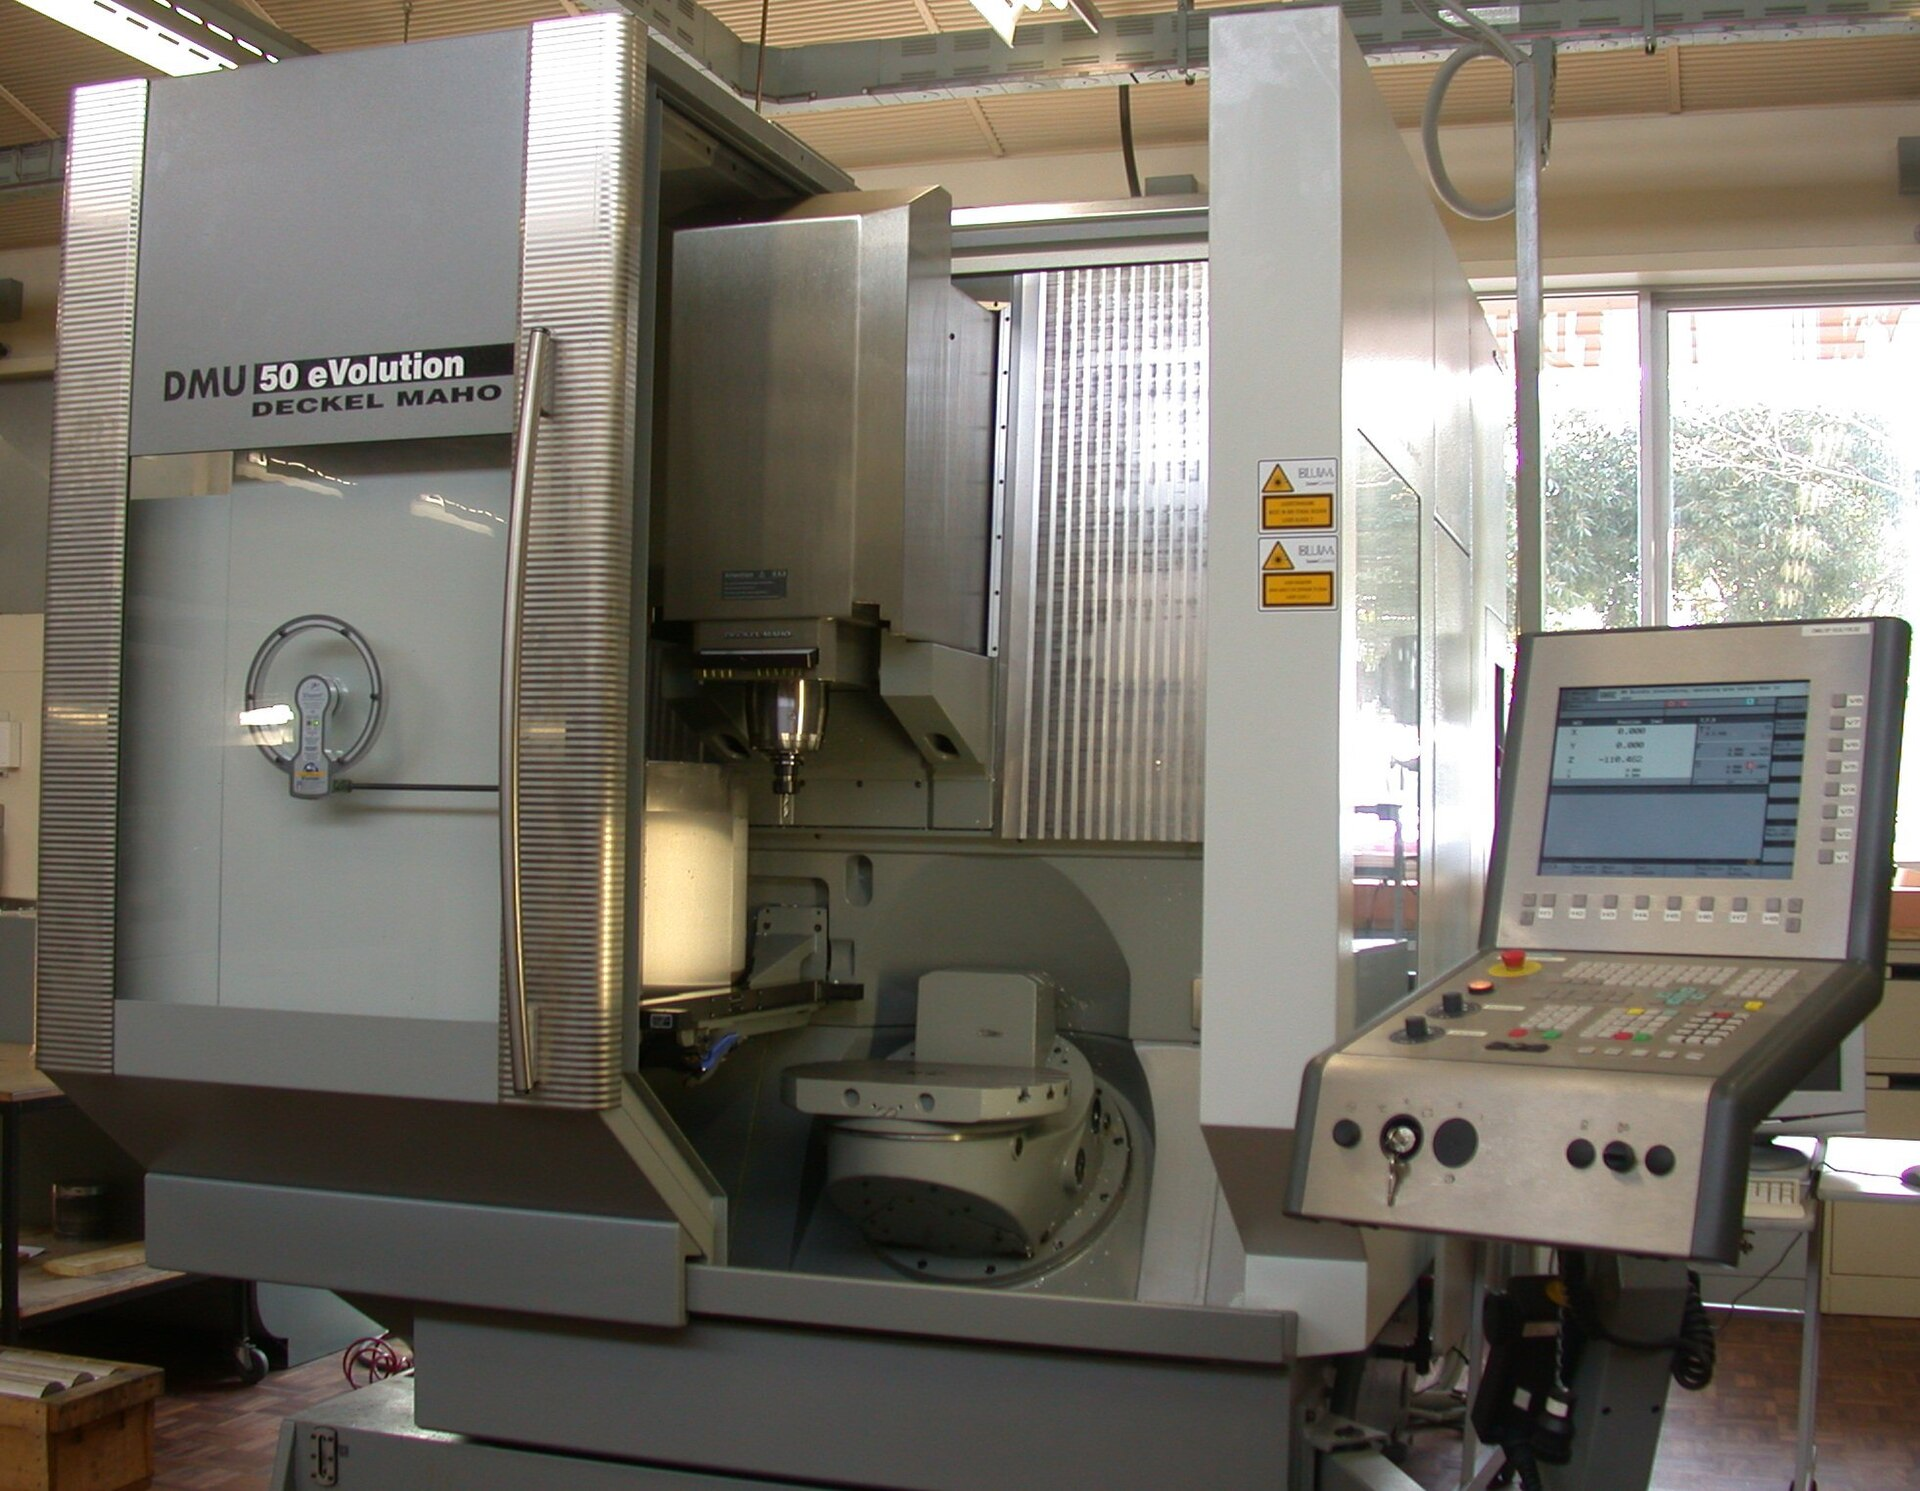
\includegraphics[width=\linewidth,height=2.6cm,keepaspectratio]{../figures/d4_machining_center.jpg}\\
\credit{5-axis machining centre. G.\ McKechnie, CC BY-SA 2.0, via Wikimedia Commons}
\begin{itemize}\scriptsize
\item Velocity FF $\omega^*\mathrel{+}=\dot x^*$: loop no longer has to create the speed from error.
\item Torque/acceleration FF $i_q^*\mathrel{+}=\hat J\ddot x^*/k_t$: inertia no longer needs velocity error.
\item FF does \emph{not} change stability -- it acts outside the loop; accuracy depends on $\hat J$ and on smooth (S-curve) references.
\end{itemize}
\end{columns}
\end{frame}

% ---------------------------------------------------------------------
\begin{frame}{Summary 3.4 -- Cascade loops}
\begin{columns}[T,onlytextwidth]
\column{.58\textwidth}
\begin{keybox}[Key take-aways]
\small
\begin{itemize}
\item Cascade: position (P) $\to$ velocity (PI) $\to$ current (PI), bandwidths separated.
\item Current PI: $T_i=L/R$, $K_p=L/(2T_\sigma)$ (TO) $\Rightarrow$ $\approx\SI{850}{Hz}$ crossover at \SI{16}{kHz}.
\item Velocity PI: symmetric optimum $\omega_c=1/(aT_\text{eq})$, prefilter for steps.
\item P position loop: following error $v/k_v$.
\item Limits require anti-windup; S-curves limit jerk.
\item Velocity + torque feedforward reduce following error by orders of magnitude.
\end{itemize}
\end{keybox}
\column{.38\textwidth}
\begin{notebox}
\textbf{Self-check}\\
1.\ $L=\SI{6}{mH}$, $T_\sigma=\SI{100}{\micro s}$: TO gain?\ (\SI{30}{V/A})\\[1mm]
2.\ Following error at $v=\SI{0.2}{m/s}$, $k_v=\SI{40}{s^{-1}}$?\ (\SI{5}{mm})\\[1mm]
3.\ Why is a prefilter needed with SO tuning?
\end{notebox}
\end{columns}
\end{frame}

% =====================================================================
\section{3.5 Loop Tuning and Bandwidth}
% =====================================================================

\begin{frame}[t]{Tuning procedure: from the inside out}
\begin{columns}[T,onlytextwidth]
\column{.42\textwidth}
\centering
\begin{tikzpicture}[node distance=2.5mm,every node/.style={font=\scriptsize}]
  \node[blk,minimum width=46mm,text width=44mm] (a) {1.\ Parameters: $R$, $L_d$, $L_q$, $\psi_\text{PM}$, $p$, angle offset};
  \node[blk,minimum width=46mm,text width=44mm,below=of a] (b) {2.\ Current loop: TO, check step \& FRF};
  \node[blk,minimum width=46mm,text width=44mm,below=of b] (c) {3.\ Inertia identification ($\hat J$)};
  \node[blk,minimum width=46mm,text width=44mm,below=of c] (d) {4.\ Velocity loop: SO / gain sweep; filters, notch};
  \node[blk,minimum width=46mm,text width=44mm,below=of d] (e) {5.\ Position loop: $k_v$, no overshoot};
  \node[blko,minimum width=46mm,text width=44mm,below=of e] (f) {6.\ Feedforward ($\dot x^*$, $\hat J\ddot x^*$, friction)};
  \foreach \u/\v in {a/b,b/c,c/d,d/e,e/f}{\draw[sig] (\u) -- (\v);}
  \draw[fb] (f.west) -- ++(-.35,0) |- node[pos=.25,left,lab,align=right]{re-check\\after\\changes} (d.west);
\end{tikzpicture}
\column{.56\textwidth}
\begin{itemize}\small
\item Each outer loop is designed on the \hl{closed} inner loop -- tune outer before inner and you tune against the wrong plant.
\item Measure, do not guess: auto-tuning routines identify $R,L$ (voltage steps), $\hat J$ (acceleration test: $\hat J=k_t\,\Delta i_q/\Delta\dot\omega$) and FRFs.
\item Increase gains until a margin limit is hit (PM $\ge45^\circ$, GM $\ge6$\,dB, $|S|_\text{max}\le 2$, i.e.\ 6\,dB), then back off.
\item Check large-signal behaviour last (limits, anti-windup, saturation of $L$).
\item Record final FRFs as a commissioning baseline.
\end{itemize}
\src{[Ellis, 2012]; [Åström \& Hägglund, 2006]}
\end{columns}
\end{frame}

% ---------------------------------------------------------------------
\begin{frame}[t]{Bandwidth separation: rule of thumb 3--10$\times$}
\begin{columns}[T,onlytextwidth]
\column{.55\textwidth}
\begin{tikzpicture}
\begin{axis}[mkplot,width=8.0cm,height=5.4cm,xmin=0,xmax=12,ymin=0,ymax=1.6,xlabel={time (ms)},ylabel={$\omega/\omega^*$},legend pos=south east]
\addplot[mkRed,thick] table[x=t,y=r1p5]{data/bwsep_step.dat};
\addplot[mkOrange,thick] table[x=t,y=r3]{data/bwsep_step.dat};
\addplot[mkMid,thick,dashed] table[x=t,y=r5]{data/bwsep_step.dat};
\addplot[mkBlue,thick] table[x=t,y=r10]{data/bwsep_step.dat};
\legend{$\omega_i/\omega_c=1.5$,$3$,$5$,$10$}
\end{axis}
\end{tikzpicture}\\
\scriptsize Computed: velocity PI designed for $\omega_c=\SI{1000}{rad/s}$ \emph{assuming an ideal current loop} ($K_p=J\omega_c/k_t$, $T_i=4/\omega_c$, prefilter); the real inner loop is $1/(1+s/\omega_i)$.
\column{.43\textwidth}
\begin{itemize}\small
\item A first-order inner loop with bandwidth $\omega_i$ costs $\arctan(\omega_c/\omega_i)$ phase at the outer crossover:
\end{itemize}
\footnotesize
\begin{tabular}{@{}cc@{}}
\toprule
$\omega_i/\omega_c$ & phase lost\\
\midrule
1.5 & $33.7^\circ$\\
3 & $18.4^\circ$\\
5 & $11.3^\circ$\\
10 & $5.7^\circ$\\
\bottomrule
\end{tabular}
\begin{itemize}\scriptsize
\item Below 3$\times$: outer design must include the inner dynamics explicitly (as SO does via $T_\text{eq}$).
\item Above 10$\times$: wasteful -- the outer loop could be faster.
\end{itemize}
\end{columns}
\end{frame}

% ---------------------------------------------------------------------
\begin{frame}[t]{Effect of the load inertia ratio}
\begin{columns}[T,onlytextwidth]
\column{.55\textwidth}
\begin{tikzpicture}
\begin{axis}[mkplot,width=8.0cm,height=5.2cm,xmin=0,xmax=20,ymin=0,ymax=1.7,xlabel={time (ms)},ylabel={$\omega/\omega^*$},legend style={at={(0.5,1.02)},anchor=south},legend columns=4]
\addplot[mkRed,thick] table[x=t,y=r0]{data/inertia_step.dat};
\addplot[mkBlue,thick] table[x=t,y=r3]{data/inertia_step.dat};
\addplot[mkOrange,thick,dashed] table[x=t,y=r10]{data/inertia_step.dat};
\addplot[mkMid,thick,dotted] table[x=t,y=r30]{data/inertia_step.dat};
\legend{$J_L/J_m=0$,$3$ (design),$10$,$30$}
\end{axis}
\end{tikzpicture}\\
\scriptsize Gains fixed (SO, $a=2$, designed for ratio 3). Computed open-loop crossover / PM:
0: \SI{439}{Hz}/$12^\circ$;\ 3: \SI{164}{Hz}/$35^\circ$;\ 10: \SI{80}{Hz}/$31^\circ$;\ 30: \SI{43}{Hz}/$21^\circ$.
\column{.43\textwidth}
\begin{itemize}\small
\item Loop gain $\propto K_{p\omega}k_t/J$: the same gains give a \hl{lower crossover} with more load inertia and a higher one (towards the delays!) with less.
\item Rule: retune with $\hat J$; adaptive gain scaling $K_{p\omega}\propto\hat J$.
\item Typical recommendation: $J_L/J_m\le 3\ldots10$ for high dynamics -- otherwise gearbox or larger motor.
\end{itemize}
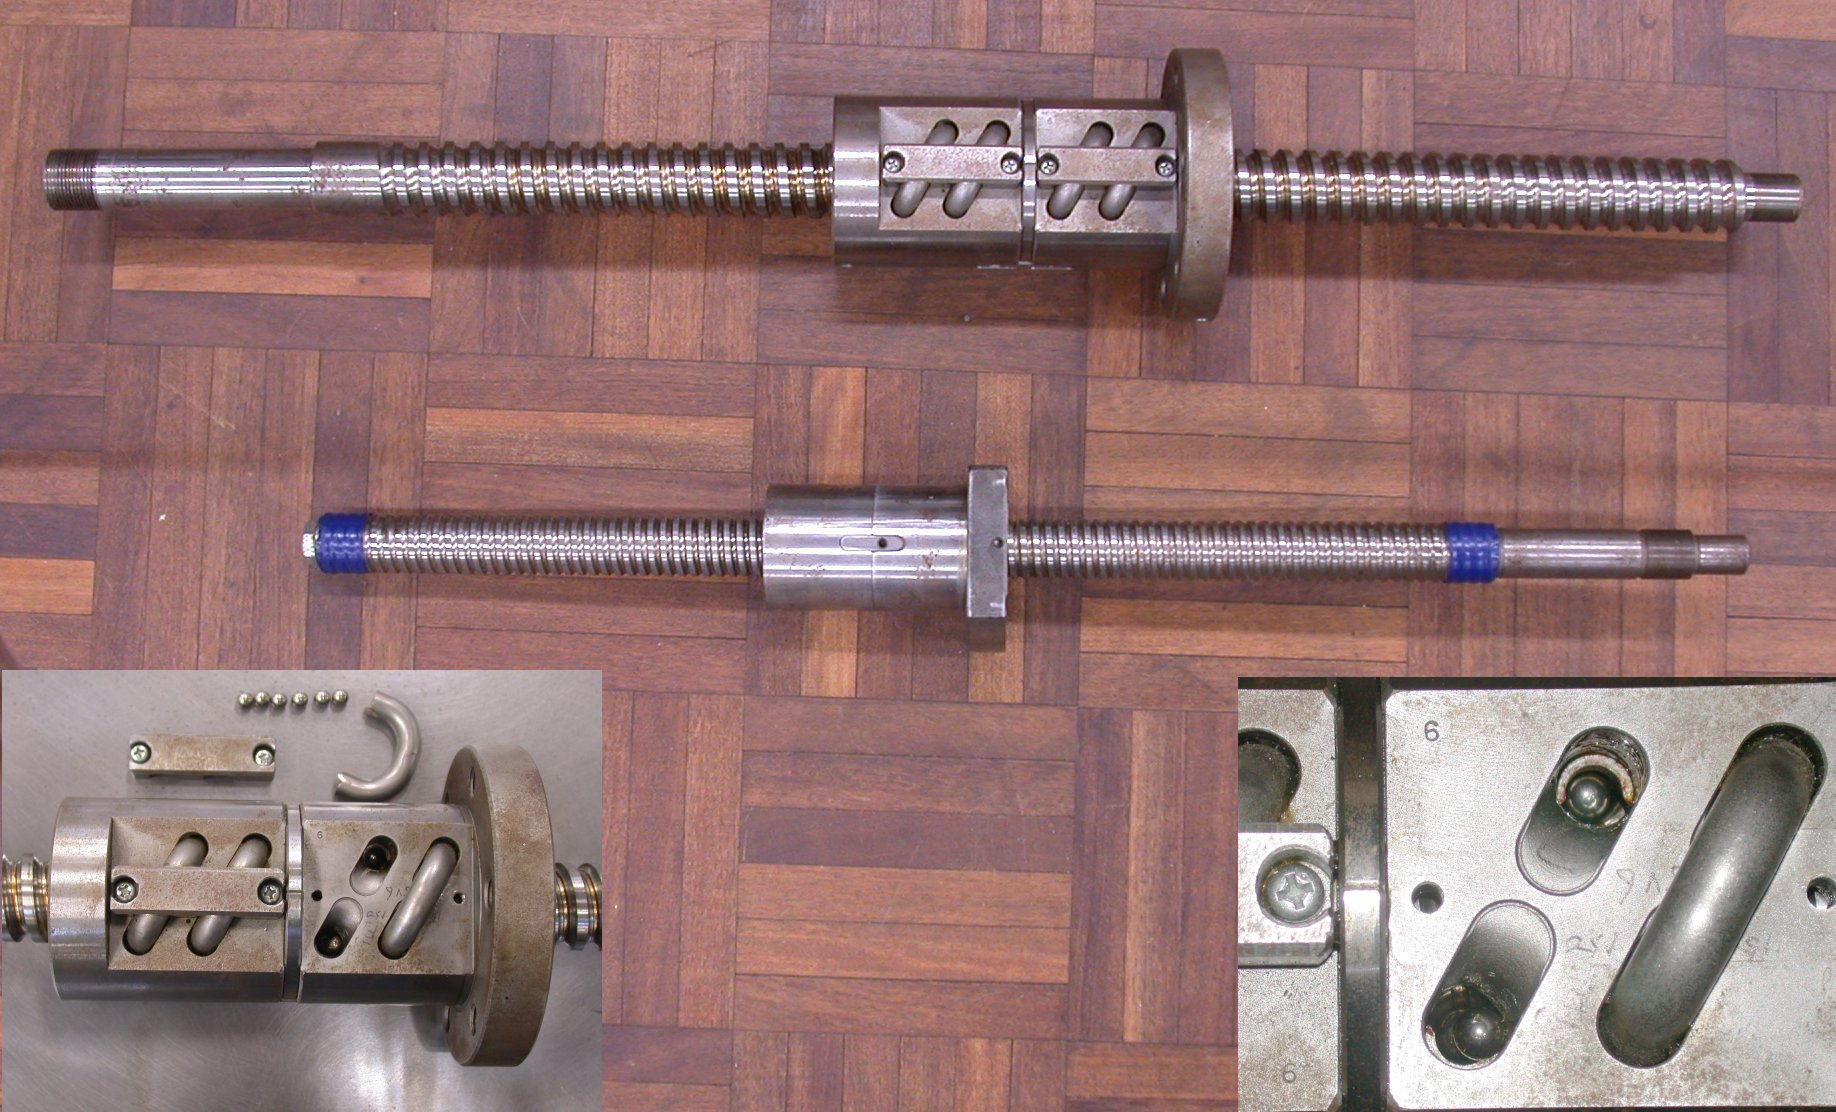
\includegraphics[width=.85\linewidth,height=1.3cm,keepaspectratio]{../figures/d4_ballscrew.jpg}\\
\credit{Ball screws. Graibeard, CC BY-SA 3.0, via Wikimedia Commons}
\end{columns}
\end{frame}

% ---------------------------------------------------------------------
\begin{frame}[t]{Delays and their phase cost at crossover}
\begin{columns}[T,onlytextwidth]
\column{.50\textwidth}
\begin{tikzpicture}
\begin{axis}[mkplot,width=7.6cm,height=5.0cm,xmode=log,xmin=10,xmax=3000,ymin=0,ymax=180,ytick={0,30,...,180},
  xlabel={crossover frequency (Hz)},ylabel={phase lag (deg)},legend pos=north west]
\addplot[mkSky,thick,domain=10:3000,samples=60] {360*x*50e-6};
\addplot[mkBlue,thick,domain=10:3000,samples=60] {360*x*100e-6};
\addplot[mkOrange,thick,domain=10:3000,samples=60] {360*x*250e-6};
\addplot[mkRed,thick,domain=10:3000,samples=60] {360*x*500e-6};
\legend{\SI{50}{\micro s},\SI{100}{\micro s},\SI{250}{\micro s},\SI{500}{\micro s}}
\end{axis}
\end{tikzpicture}\\
\scriptsize Pure delay $e^{-sT_d}$: $\Delta\varphi=360^\circ\,f_c\,T_d$ -- linear in $f$, no magnitude change.
\column{.48\textwidth}
\footnotesize
\begin{tabularx}{\linewidth}{@{}X r@{}}
\toprule
\textbf{Delay source} & \textbf{typical}\\
\midrule
Computation (1 sample at \SI{16}{kHz}) & \SI{62.5}{\micro s}\\
PWM / ZOH ($T_s/2$) & \SI{31}{\micro s}\\
Current sensing, $\Sigma\Delta$ decimation & 5--20\,\si{\micro s}\\
Encoder serial protocol & 10--30\,\si{\micro s}\\
Velocity filter ($T_f$) & 0.1--1\,ms\\
Field bus (set-point, 1 cycle) & 0.125--1\,ms\\
\bottomrule
\end{tabularx}\\[2mm]
\begin{keybox}[Example]
\scriptsize Velocity loop, $T_\text{eq}=\SI{0.5}{ms}$ at $f_c=\SI{160}{Hz}$: $28.8^\circ$ lost. Halving $T_f$ or doubling $f_s$ buys phase that can be traded for bandwidth.
\end{keybox}
\end{columns}
\end{frame}

% ---------------------------------------------------------------------
\begin{frame}[t]{Technical optimum vs.\ symmetric optimum}
\footnotesize
\begin{tabularx}{\linewidth}{@{}l X X@{}}
\toprule
 & \textbf{Technical (magnitude) optimum, TO} & \textbf{Symmetric optimum, SO}\\
\midrule
Plant type & $\dfrac{K}{(1+sT_1)(1+sT_\sigma)}$,\ $T_1\gg T_\sigma$ & $\dfrac{K}{sT_I\,(1+sT_\sigma)}$ (integrating)\\[2mm]
PI choice & $T_i=T_1$,\ $K_p=\dfrac{T_1}{2KT_\sigma}$ & $T_i=a^2T_\sigma$,\ $K_p=\dfrac{T_I}{aKT_\sigma}$\\[2mm]
Closed loop & $\approx\dfrac{1}{1+2T_\sigma s+2T_\sigma^2s^2}$, $\zeta=0.707$ & zero at $1/T_i$, needs prefilter\\[1mm]
Step response & 4.3\,\% overshoot, $t_r\approx4.7\,T_\sigma$ & 43\,\% ($a=2$), 8\,\% with prefilter\\
Phase margin & $\approx65^\circ$ & $\arctan\frac{a^2-1}{2a}$ (37$^\circ$ at $a=2$)\\
Disturbance rejection & slow for $T_1\gg T_\sigma$ (pole cancelled) & good: no cancellation\\
Used for & \textbf{current loop} ($T_1=L/R$) & \textbf{velocity loop} (inertia $=$ integrator)\\
\bottomrule
\end{tabularx}
\vspace{2mm}
\begin{columns}[T,onlytextwidth]
\column{.5\textwidth}
\begin{notebox}
Both are \emph{starting points} from German drive practice (Kessler, 1955/58). Industrial auto-tuners do similar things in the frequency domain with explicit PM/GM targets.
\end{notebox}
\column{.48\textwidth}
\begin{notebox}
For the velocity loop many practitioners use $a=2.5\ldots4$ (PM 45--60$^\circ$) for robustness to $J$ and resonances.
\end{notebox}
\end{columns}
\end{frame}

% ---------------------------------------------------------------------
\begin{frame}[t]{Typical bandwidths of industrial servo drives}
\begin{columns}[T,onlytextwidth]
\column{.56\textwidth}
\footnotesize
\begin{tabularx}{\linewidth}{@{}X l l@{}}
\toprule
\textbf{Loop} & \textbf{closed-loop BW} & \textbf{limited by}\\
\midrule
Current & 1--3\,kHz & $f_s$, PWM delay\\
Velocity & 100--500\,Hz (rigid) & filters, resonance\\
& 20--100\,Hz (compliant) & \\
Position & 10--100\,Hz & velocity loop, overshoot\\
\midrule
Machine-tool $k_v$ & 1--6\,(m/min)/mm & 17--100\,s$^{-1}$\\
\bottomrule
\end{tabularx}\\[2mm]
\scriptsize Order-of-magnitude values from drive manuals and the literature [Ellis, 2012]; the achievable values depend on the mechanics far more than on the drive.
\begin{itemize}\scriptsize
\item Robots: velocity BW limited by gear compliance (strain wave gears) to a few tens of Hz per joint.
\item Direct drives (linear/torque motors): velocity BW several hundred Hz.
\end{itemize}
\column{.42\textwidth}
\centering
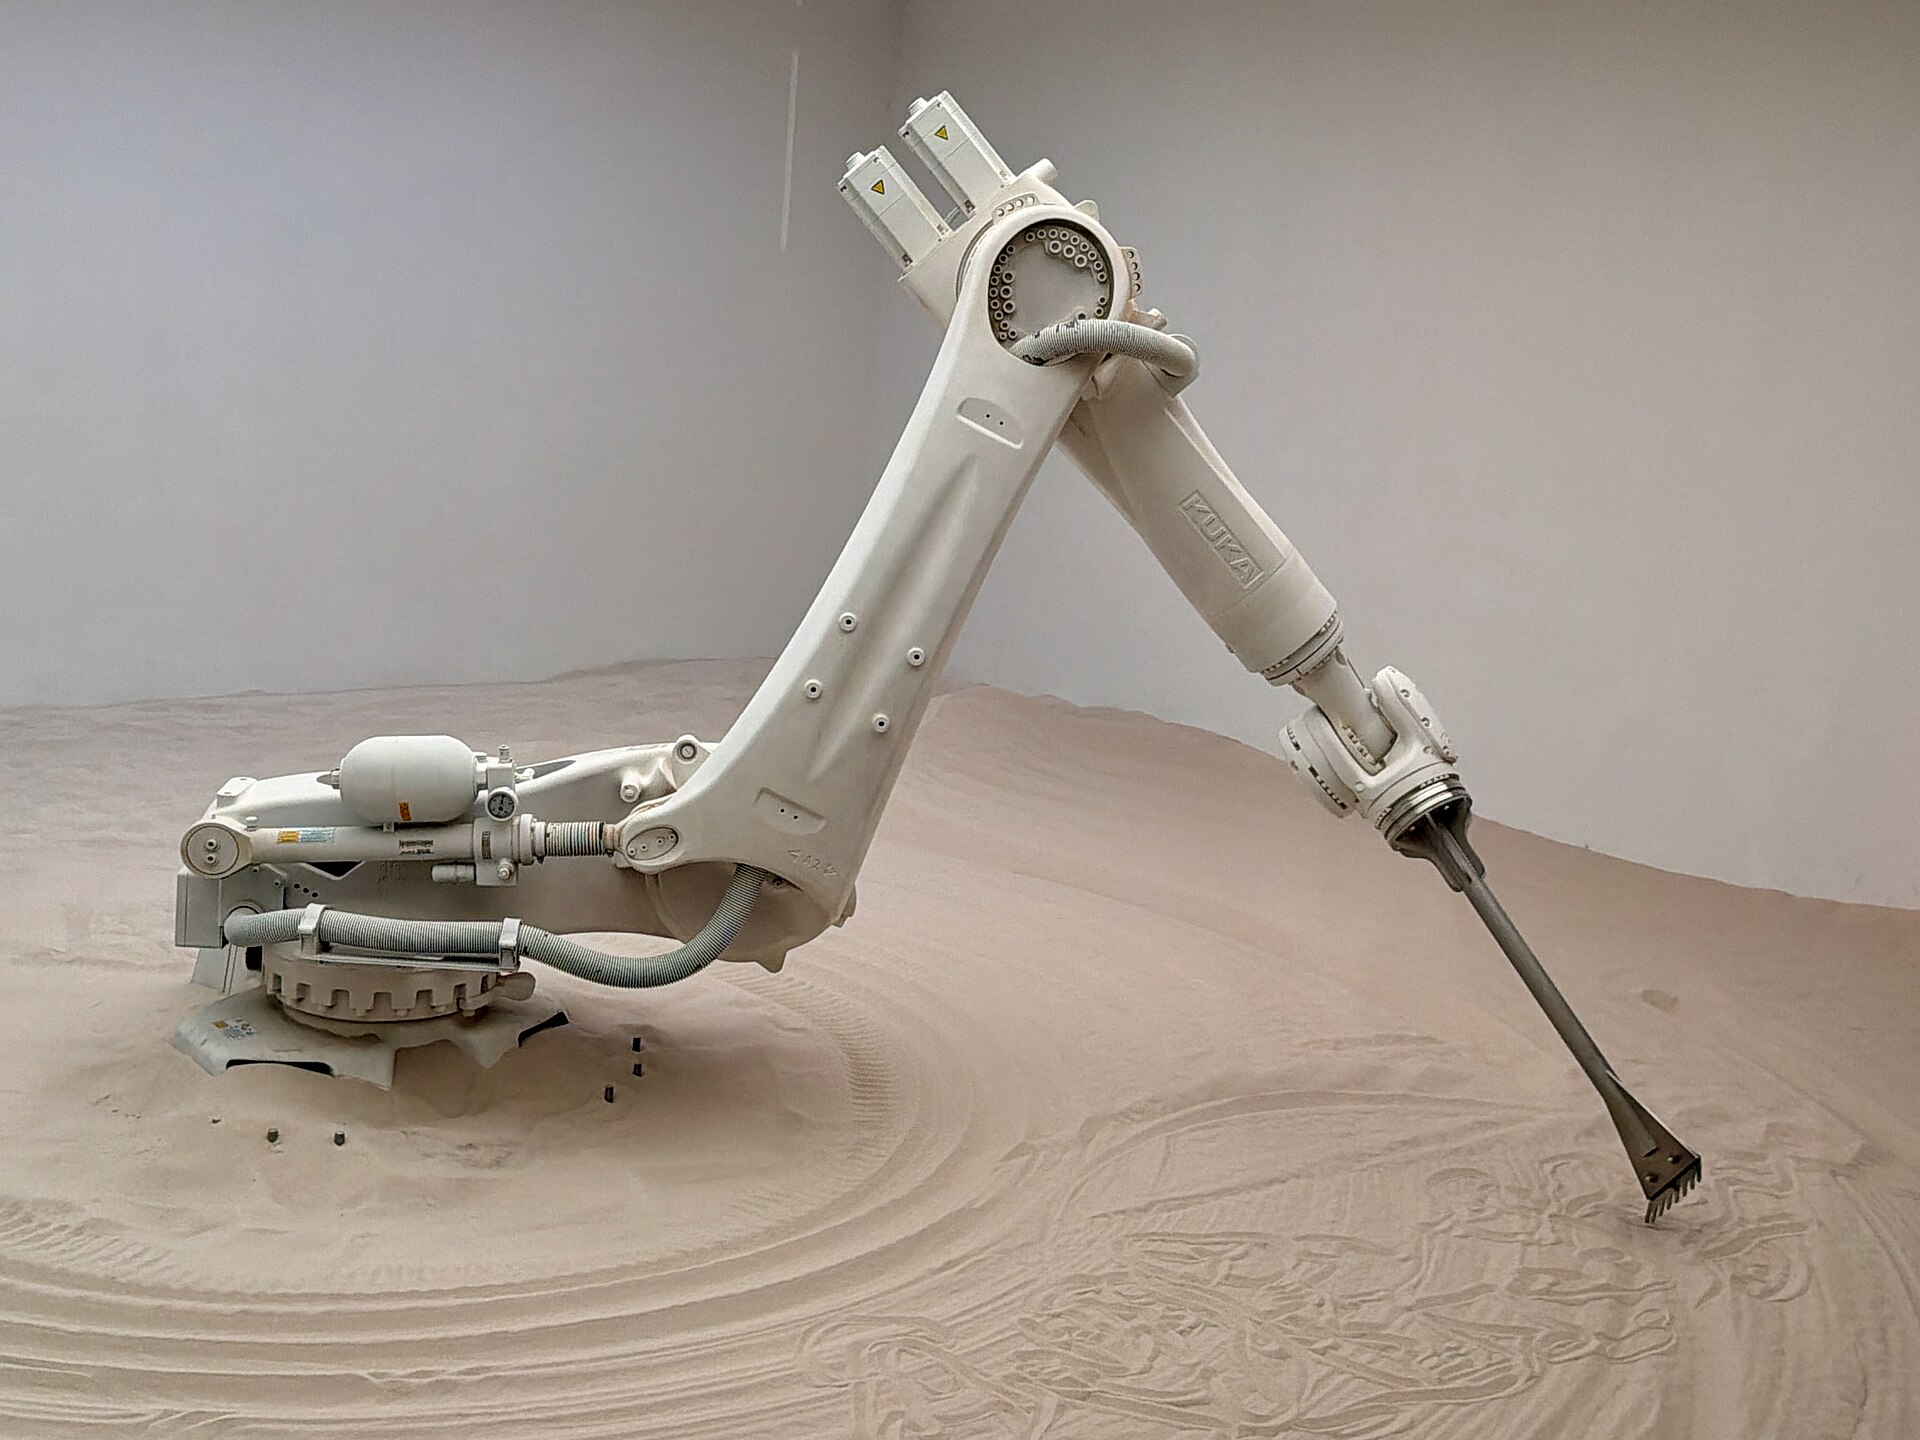
\includegraphics[width=\linewidth,height=4.3cm,keepaspectratio]{../figures/d4_kuka_robot.jpg}\\
\credit{Industrial robot. Oleg Yunakov, CC BY-SA 4.0, via Wikimedia Commons}
\end{columns}
\end{frame}

% ---------------------------------------------------------------------
\begin{frame}[t]{Measuring frequency response functions (FRFs)}
\begin{columns}[T,onlytextwidth]
\column{.56\textwidth}
\centering
\begin{tikzpicture}[x=1cm,y=1cm]
  \node[sumn] (s1) at (0.6,1) {};
  \node[blk] (c) at (1.9,1) {$C(s)$};
  \node[sumn] (s2) at (3.3,1) {};
  \node[blk] (g) at (4.7,1) {$G(s)$};
  \draw[sig] (-.2,1) node[left,lab]{$r$} -- (s1); \draw[sig] (s1) -- (c); \draw[sig] (c) -- node[above,lab]{$c$} (s2);
  \draw[sig] (s2) -- node[above,lab]{$u$} (g); \draw[sig] (g) -- (6.3,1) node[right,lab]{$y$};
  \draw[fb] (5.9,1) -- (5.9,0) -| (s1.south);
  \draw[ff] (3.3,2.1) node[above,lab]{injection $d$ (sweep / chirp / PRBS)} -- (s2.north);
  \node[font=\tiny,mkGray] at (.45,.65) {$-$};
\end{tikzpicture}
\begin{eqbox}\small\centering
$G=\dfrac{Y}{U},\qquad S=\dfrac{U}{D},\qquad L=-\dfrac{C}{U}=\dfrac1S-1$
\end{eqbox}
\begin{itemize}\scriptsize
\item Excite \emph{inside} the closed loop (machine stays under control); estimate with cross-spectra $\hat G=\hat S_{uy}/\hat S_{uu}$, average, check \term{coherence} $\gamma^2\approx1$.
\item Injection at current reference $\Rightarrow$ mechanical plant ($k_t/Js$ + resonances); at velocity reference $\Rightarrow$ closed-loop BW.
\item Amplitude: large enough above friction/noise, small enough to stay linear (no current limit).
\end{itemize}
\column{.42\textwidth}
\centering
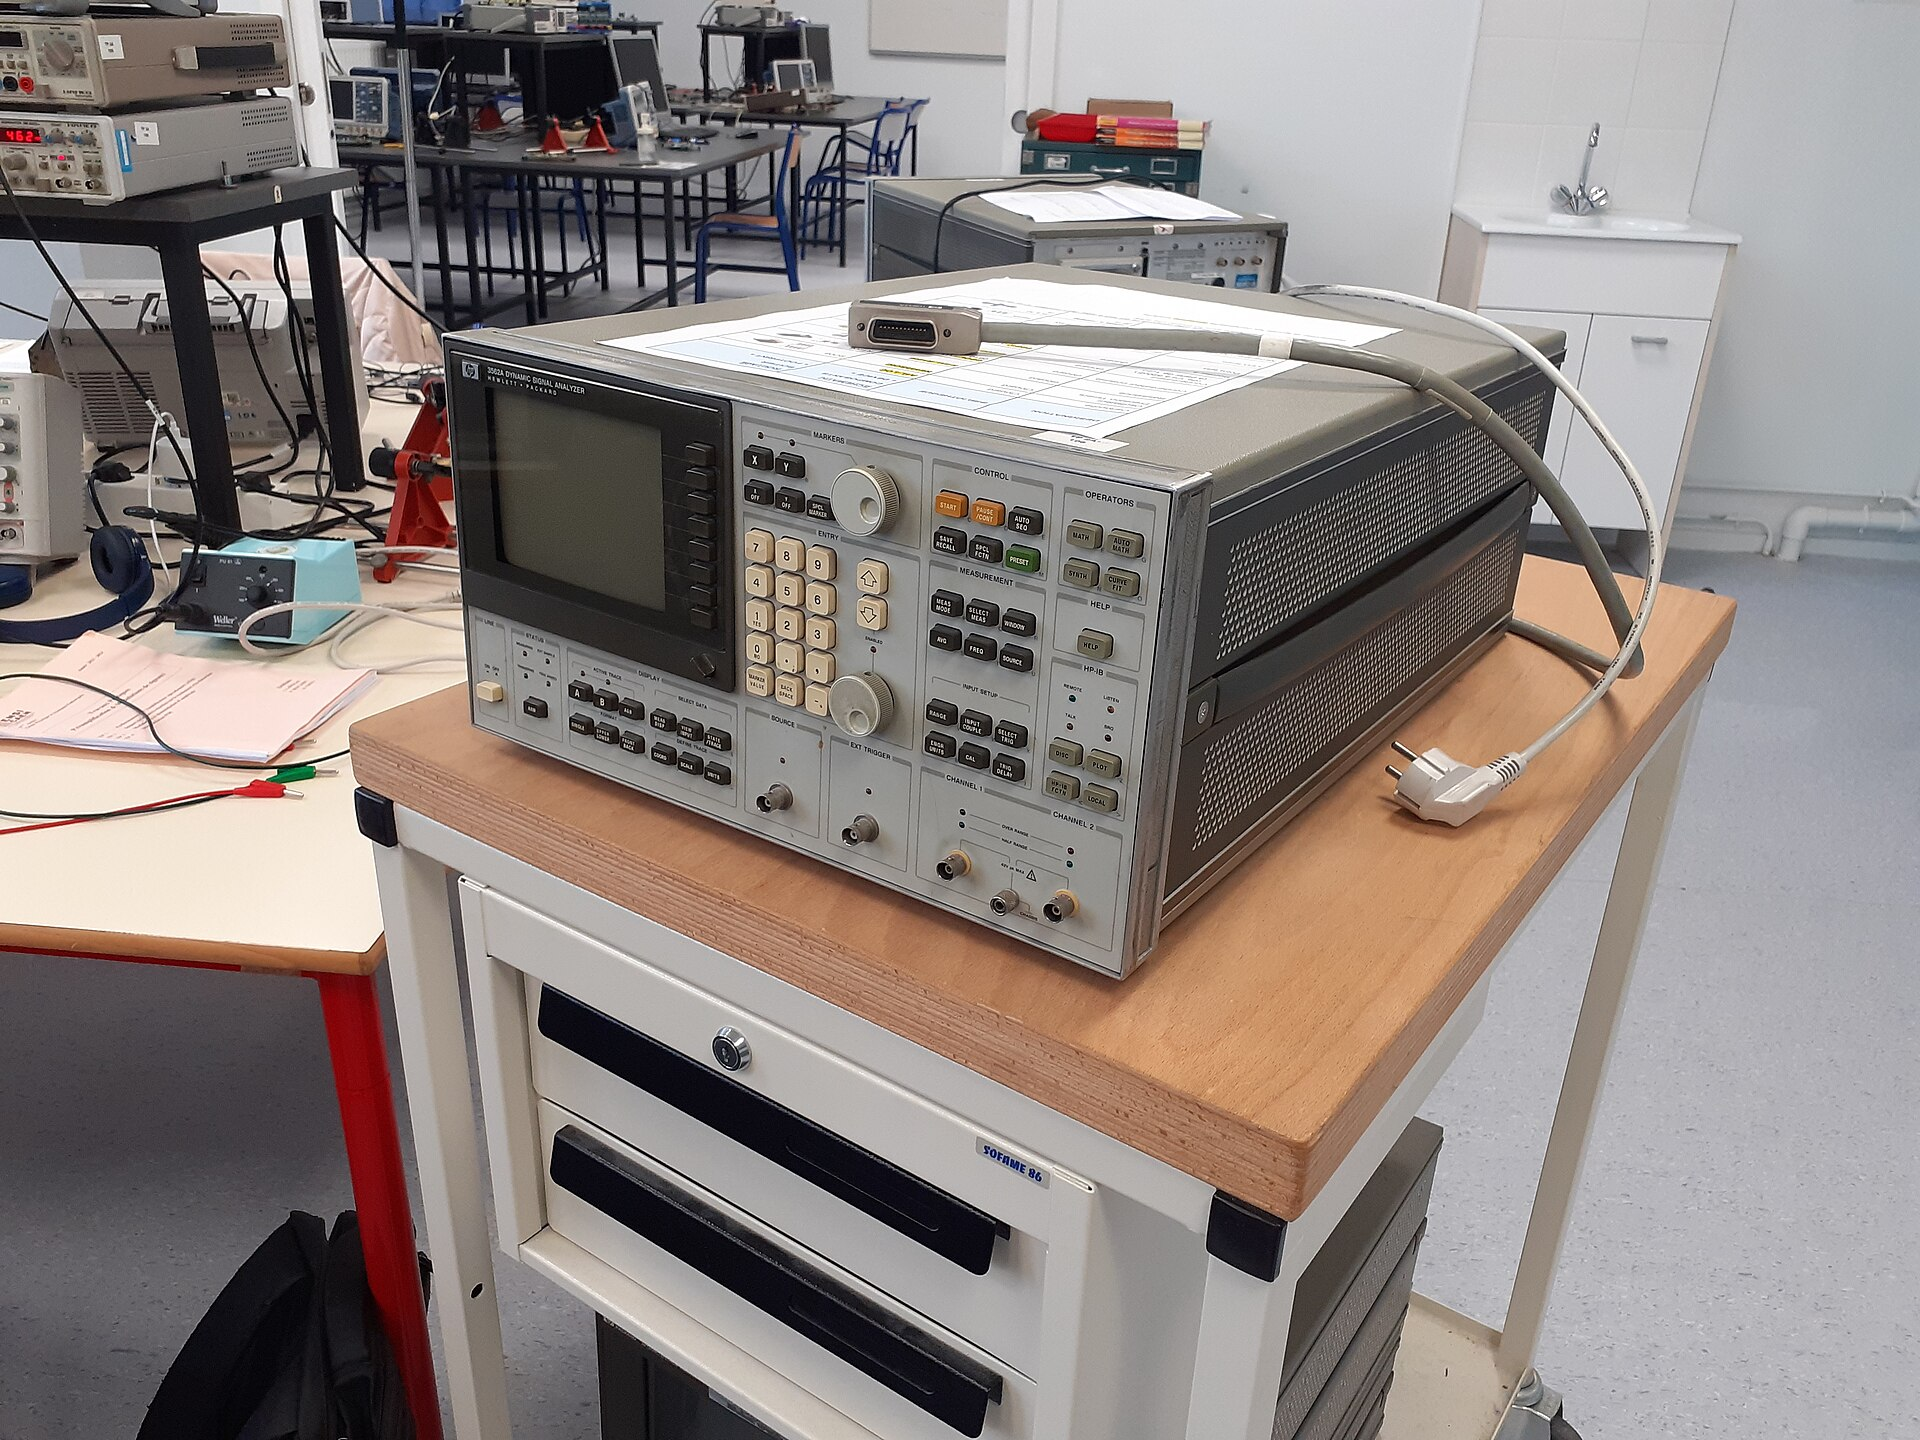
\includegraphics[width=\linewidth,height=3.2cm,keepaspectratio]{../figures/d4_signal_analyzer.jpg}\\
\credit{HP 3562A dynamic signal analyzer. Loxyger, CC BY 4.0, via Wikimedia Commons}\\[1mm]
\begin{notebox}
Modern drives have this analyzer built in: the commissioning software injects a chirp and plots Bode diagrams directly.
\end{notebox}
\end{columns}
\end{frame}

% ---------------------------------------------------------------------
\begin{frame}[t]{A measured-style FRF: two-mass resonance and notch filter}
\begin{columns}[T,onlytextwidth]
\column{.56\textwidth}
\begin{tikzpicture}
\begin{groupplot}[group style={group size=1 by 2,vertical sep=3mm,xticklabels at=edge bottom},
  mkplot,width=8.2cm,xmode=log,xmin=10,xmax=3000,legend pos=south west]
\nextgroupplot[height=3.9cm,ylabel={$|\omega_m/i_q|$ (dB)},ymin=-10,ymax=70]
\addplot[mkGray,thick,dashed] table[x=f,y=mR]{data/frf.dat};
\addplot[mkBlue,thick] table[x=f,y=mG]{data/frf.dat};
\addplot[mkOrange,thick] table[x=f,y=mGN]{data/frf.dat};
\legend{rigid $k_t/(J_\Sigma s)$,two-mass,with notch}
\nextgroupplot[height=2.8cm,ylabel={$\angle$ (deg)},xlabel={frequency (Hz)},ymin=-185,ymax=5,ytick={-180,-90,0}]
\addplot[mkBlue,thick] table[x=f,y=pG]{data/frf.dat};
\end{groupplot}
\end{tikzpicture}
\column{.42\textwidth}
\scriptsize Computed: $J_m=\SI{3e-4}{}$, $J_L=\SI{9e-4}{kg\,m^2}$, $k_s=\SI{3200}{Nm/rad}$, 3\,\% damping.
\begin{itemize}\scriptsize
\item Anti-resonance $f_a=\frac1{2\pi}\sqrt{k_s/J_L}=\SI{300}{Hz}$, resonance $f_r=f_a\sqrt{1+J_L/J_m}=\SI{600}{Hz}$.
\item Above $f_r$ the motor ``sees'' only $J_m$: gain jumps by $1+J_L/J_m$ (12\,dB) $\Rightarrow$ crossover may move up into the delays $\Rightarrow$ instability (``buzz'').
\item \term{Notch filter} at $f_r$ (in the current reference): $N(s)=\dfrac{s^2+2\zeta_z\omega_rs+\omega_r^2}{s^2+2\zeta_p\omega_rs+\omega_r^2}$, here $\zeta_z=0.05$, $\zeta_p=0.5$.
\item Notch costs phase below $f_r$; resonances move with load $\Rightarrow$ deeper treatment on Day 5.
\end{itemize}
\end{columns}
\end{frame}

% ---------------------------------------------------------------------
\begin{frame}{Summary 3.5 -- Tuning and bandwidth}
\begin{columns}[T,onlytextwidth]
\column{.58\textwidth}
\begin{keybox}[Key take-aways]
\small
\begin{itemize}
\item Tune inside out; each loop on the closed inner loop.
\item Separate bandwidths 3--10$\times$; less needs explicit modelling.
\item The inertia ratio scales the velocity-loop gain: retune with $\hat J$.
\item Every delay costs $360^\circ f_cT_d$ -- budget them.
\item TO for the current loop, SO for the velocity loop as starting points.
\item Measure FRFs in closed loop; watch coherence, resonances, notches.
\end{itemize}
\end{keybox}
\column{.38\textwidth}
\begin{notebox}
\textbf{Self-check}\\
1.\ Phase lost by \SI{200}{\micro s} at \SI{250}{Hz}?\ ($18^\circ$)\\[1mm]
2.\ Inertia ratio doubles: what happens to $\omega_c$ with fixed gains?\\[1mm]
3.\ Why inject at the controller output rather than open the loop?
\end{notebox}
\end{columns}
\end{frame}

% =====================================================================
\section{3.6 Disturbances and Compensation}
% =====================================================================

\begin{frame}[t]{Disturbances: load torque and friction}
\begin{columns}[T,onlytextwidth]
\column{.50\textwidth}
\begin{tikzpicture}
\begin{axis}[mkplot,width=7.4cm,height=5.0cm,xmin=-20,xmax=20,ymin=-0.32,ymax=0.32,
  xlabel={$\omega$ (rad/s)},ylabel={friction torque $T_f$ (Nm)},legend pos=north west,
  yticklabel style={/pgf/number format/fixed}]
\addplot[mkBlue,line width=1.1pt,domain=0.01:20,samples=120] {0.1+0.06*exp(-(x/2)^2)+0.005*x};
\addplot[mkBlue,line width=1.1pt,domain=-20:-0.01,samples=120,forget plot] {-(0.1+0.06*exp(-(x/2)^2))+0.005*x};
\addplot[mkOrange,thick,dashed,domain=0.01:20,samples=2] {0.1+0.005*x};
\addplot[mkOrange,thick,dashed,domain=-20:-0.01,samples=2,forget plot] {-0.1+0.005*x};
\addplot[mkBlue,thick,forget plot] coordinates {(0,-0.16) (0,0.16)};
\legend{Stribeck model,Coulomb + viscous}
\end{axis}
\end{tikzpicture}\\
\scriptsize $T_f=\operatorname{sign}(\omega)\big[T_C+(T_S-T_C)e^{-(\omega/\omega_S)^2}\big]+B\omega$; here $T_C=\SI{0.1}{Nm}$, $T_S=\SI{0.16}{Nm}$, $\omega_S=\SI{2}{rad/s}$, $B=\SI{5}{mNm\,s/rad}$.
\column{.48\textwidth}
\begin{itemize}\small
\item Mechanics: $J\dot\omega=k_ti_q-T_L-T_f(\omega)$.
\item \term{Load torque} $T_L$: process forces, gravity (vertical axes!), cutting forces.
\item \term{Friction}: discontinuous at $\omega=0$ $\Rightarrow$ stick-slip, quadrant glitches on circles, limit cycles with integral action.
\item PI rejects a step $T_L$ with zero steady-state error, but the transient dip depends on $\omega_c$ and $J$.
\item Other disturbances: cogging and ripple torque, dead-time voltage error, measurement noise, cable forces.
\end{itemize}
\src{[Armstrong-Hélouvry, Dupont \& Canudas de Wit, 1994]}
\end{columns}
\end{frame}

% ---------------------------------------------------------------------
\begin{frame}[t]{Feedforward: velocity, acceleration/torque and friction}
\centering
\begin{tikzpicture}[x=1cm,y=1cm]
  \node[blko,minimum width=14mm] (tg) at (0,0) {trajectory\\$x^*,\dot x^*,\ddot x^*$};
  \node[sumn] (s1) at (1.9,0) {};
  \node[blk] (kv) at (3.0,0) {$k_v$};
  \node[sumn] (s2) at (4.2,0) {};
  \node[sumn] (s3) at (5.0,0) {};
  \node[blk] (pi) at (6.2,0) {PI$_\omega$};
  \node[sumn] (s4) at (7.4,0) {};
  \node[blk] (cl) at (8.7,0) {current\\loop $\cdot k_t$};
  \node[blk] (pl) at (10.6,0) {$\dfrac{1}{Js}$};
  \node[blk,minimum width=8mm] (in) at (12.1,0) {$\dfrac1s$};
  \draw[sig] (tg) -- (s1); \draw[sig] (s1) -- (kv); \draw[sig] (kv) -- (s2); \draw[sig] (s2) -- (s3); \draw[sig] (s3) -- (pi);
  \draw[sig] (pi) -- (s4); \draw[sig] (s4) -- (cl); \draw[sig] (cl) -- (pl); \draw[sig] (pl) -- (in); \draw[sig] (in) -- (13,0) node[right,lab]{$x$};
  \draw[fb] (12.75,0) -- (12.75,-1.2) -| (s1.south);
  \draw[fb] (11.35,0) -- (11.35,-.8) -| (s3.south);
  \draw[ff] (tg.north) |- node[pos=.75,above,lab]{$\dot x^*$ (velocity FF)} (4.2,1.0) -- (s2.north);
  \draw[ff] (tg.north) ++(.3,0) |- node[pos=.8,above,lab]{$\hat J\ddot x^*/k_t$ (acceleration / torque FF)} (7.4,1.6) -- (s4.north);
  \draw[ff] (tg.north) ++(-.3,0) |- node[pos=.85,above,lab]{$\hat T_f(\dot x^*)/k_t$ (friction FF)} (7.25,2.2) -- (7.25,0.1);
\end{tikzpicture}
\vspace{2mm}
\begin{columns}[T,onlytextwidth]
\column{.5\textwidth}
\begin{itemize}\small
\item Ideal FF inverts the plant: $u_\text{FF}=G^{-1}x^*$. For a rigid axis: $i_q^*=\big(\hat J\ddot x^*+\hat B\dot x^*+\hat T_f\big)/k_t$.
\item Requires smooth references (S-curve) -- FF of a jerk step is a torque step.
\end{itemize}
\column{.48\textwidth}
\begin{itemize}\small
\item FF acts \hl{outside the loop}: no stability change, feedback only corrects the model error.
\item Typical gains 80--100\,\% of model; check on overshoot at the end of acceleration.
\end{itemize}
\end{columns}
\end{frame}

% ---------------------------------------------------------------------
\begin{frame}[t]{Disturbance observer (DOB): basic logic}
\begin{columns}[T,onlytextwidth]
\column{.55\textwidth}
\centering
\begin{tikzpicture}[x=1cm,y=1cm]
  \node[sumn] (s0) at (0.4,1.6) {};
  \node[blk] (cl) at (1.8,1.6) {$k_t$};
  \node[sumn] (s1) at (3.1,1.6) {};
  \node[blk] (pl) at (4.4,1.6) {$\dfrac{1}{Js}$};
  \draw[sig] (-.6,1.6) node[left,lab]{$i_q^*$} -- (s0); \draw[sig] (s0) -- node[above,lab]{$i_q$} (cl);
  \draw[sig] (cl) -- node[above,lab]{$T_e$} (s1);
  \draw[sig] (s1) -- (pl); \draw[sig] (pl) -- (6.2,1.6) node[right,lab]{$\omega$};
  \draw[sig] (3.1,2.5) node[above,lab]{$T_L$ ($-$)} -- (s1.north);
  % observer
  \node[blko] (inv) at (4.4,0.2) {$\hat J s\,Q(s)$};
  \node[blko] (q) at (1.8,0.2) {$k_t\,Q(s)$};
  \node[sumn] (s2) at (3.1,-0.9) {};
  \node[blko] (g) at (1.0,-0.9) {$1/k_t$};
  \draw[fb] (5.6,1.6) |- (inv.east);
  \draw[fb] (1.0,1.6) -- (1.0,.2) -- (q.west);
  \draw[fb] (q.east) -| (s2.north);
  \draw[fb] (inv.south) |- (s2.east);
  \draw[fb] (s2.west) -- node[above,lab]{$\hat T_L$} (g.east);
  \draw[fb] (g.west) -| (s0.south);
  \node[font=\tiny,mkGray] at (3.35,-.6) {$+$}; \node[font=\tiny,mkGray] at (3.45,-1.1) {$-$};
  \node[font=\tiny,mkGray] at (.2,1.25) {$+$};
\end{tikzpicture}\\[1mm]
\scriptsize $Q(s)=\dfrac{1}{1+s\tau_Q}$ low-pass makes the inverse model $\hat Js$ proper.
\column{.43\textwidth}
\begin{itemize}\small
\item Idea: compare what the motor \emph{should} do ($k_ti_q$) with what it \emph{does} ($\hat J\dot\omega$). The difference is the lumped disturbance:
\end{itemize}
\begin{eqbox}\small\centering
$\hat T_L=Q(s)\big[k_ti_q-\hat Js\,\omega\big]$
\end{eqbox}
\begin{itemize}\scriptsize
\item Feeding $\hat T_L/k_t$ back makes the axis behave like the nominal $1/(\hat Js)$ below $1/\tau_Q$ -- load, friction and inertia error are rejected.
\item Bandwidth of $Q$ limited by noise ($s\omega$!) and delays; typical $1/\tau_Q$ = 0.5--2$\times\omega_c$.
\item $\hat T_L$ is also a useful signal: load monitoring, collision detection.
\end{itemize}
\src{[Ohnishi, Shibata \& Murakami, 1996]}
\end{columns}
\end{frame}

% ---------------------------------------------------------------------
\begin{frame}[t]{DOB vs.\ PI alone: load-torque step}
\begin{columns}[T,onlytextwidth]
\column{.56\textwidth}
\begin{tikzpicture}
\begin{groupplot}[group style={group size=1 by 2,vertical sep=3mm,xticklabels at=edge bottom},
  mkplot,width=8.2cm,xmin=0,xmax=30,legend pos=south east]
\nextgroupplot[height=3.8cm,ylabel={$\omega$ (rad/s)},ymin=-2.1,ymax=.4]
\addplot[mkRed,thick] table[x=t,y=w_pi]{data/dob.dat};
\addplot[mkBlue,thick] table[x=t,y=w_dob]{data/dob.dat};
\legend{PI only,PI + DOB}
\nextgroupplot[height=2.9cm,ylabel={$\hat T_L$ (Nm)},xlabel={time (ms)},ymin=-.2,ymax=2.4]
\addplot[mkOrange,thick] table[x=t,y=dhat]{data/dob.dat};
\addplot[mkGray,dashed] coordinates {(0,0) (5,0) (5,2) (30,2)};
\end{groupplot}
\end{tikzpicture}
\column{.42\textwidth}
\scriptsize Simulated: reference motor, velocity PI (SO, $a=3$) holding $\omega^*=0$, load step $T_L=\SI{2}{Nm}$ at \SI{5}{ms}; DOB with $\tau_Q=\SI{0.5}{ms}$, $\hat J=J$.
\begin{itemize}\small
\item Peak speed dip: \SI{1.85}{rad/s} $\to$ \SI{0.70}{rad/s} (2.6$\times$ better), and recovery is faster.
\item The estimate $\hat T_L$ converges to the true \SI{2}{Nm} within $\approx3\tau_Q$ plus loop delays.
\item Same effect could be obtained with more PI gain -- but that would cost phase margin and noise; DOB adds rejection \hl{without} changing the reference response (nominal).
\end{itemize}
\end{columns}
\end{frame}

% ---------------------------------------------------------------------
\begin{frame}[t]{Cogging and torque ripple compensation (brief)}
\begin{columns}[T,onlytextwidth]
\column{.55\textwidth}
\begin{tikzpicture}
\begin{axis}[mkplot,width=8.0cm,height=5.0cm,xmin=0,xmax=45,ymin=-.1,ymax=.1,xtick={0,15,30,45},
  xlabel={mechanical angle (deg)},ylabel={torque (Nm)},legend pos=south east,yticklabel style={/pgf/number format/fixed}]
\addplot[mkBlue,thick] table[x=th,y=Tc]{data/cogging.dat};
\addplot[mkOrange,thick] table[x=th,y=res]{data/cogging.dat};
\legend{cogging torque,residual after LUT}
\end{axis}
\end{tikzpicture}\\
\scriptsize Illustrative 12-slot/8-pole motor: fundamental cogging period $360^\circ/\text{LCM}(12,8)=15^\circ$ mech. LUT with $1^\circ$ steps, 95\,\% gain: \SI{0.146}{Nm} p-p $\to$ \SI{0.015}{Nm} p-p.
\column{.43\textwidth}
\begin{itemize}\small
\item \term{Cogging}: magnets vs.\ slot openings, present at zero current, periodic in $\theta_m$.
\item \term{Ripple}: back-EMF harmonics, current sensor offsets/gain errors (1st/2nd order in $\theta_e$), dead time (6th).
\item Compensation: measure $i_q$ needed at constant slow speed vs.\ angle $\Rightarrow$ look-up table $\Delta i_q(\theta_m)$ added to $i_q^*$; or iterative learning / repetitive control.
\item Effective at low speed, where the velocity loop cannot reject the ripple frequency $p\,n/60\times$ harmonic order.
\item Sensor offset calibration first -- it is the cheapest ripple reduction.
\end{itemize}
\end{columns}
\end{frame}

% ---------------------------------------------------------------------
\begin{frame}{Summary 3.6 -- Disturbances and compensation}
\begin{columns}[T,onlytextwidth]
\column{.58\textwidth}
\begin{keybox}[Key take-aways]
\small
\begin{itemize}
\item Load torque and friction act at the plant input; PI rejects them with limited speed.
\item Feedforward (velocity, acceleration/torque, friction) cancels \emph{known} effects outside the loop.
\item DOB estimates the \emph{unknown} lumped disturbance from $k_ti_q-\hat J\dot\omega$ and compensates it.
\item Cogging/ripple: periodic in angle $\Rightarrow$ table-based compensation.
\end{itemize}
\end{keybox}
\column{.38\textwidth}
\begin{notebox}
\textbf{Self-check}\\
1.\ Which compensation for a vertical axis with gravity load?\ (constant torque FF / integrator / DOB)\\[1mm]
2.\ Why does DOB need $Q(s)$?\\[1mm]
3.\ Cogging period of a 9-slot/6-pole motor?\ ($20^\circ$)
\end{notebox}
\end{columns}
\end{frame}

% =====================================================================
\section{Day 4 Wrap-up}
% =====================================================================

\begin{frame}[t]{Day summary}
\begin{columns}[T,onlytextwidth]
\column{.5\textwidth}
\begin{defbox}[From voltage to motion]
\scriptsize
\textbf{3.2} SVPWM synthesises $\vec v^*$ up to $V_\text{dc}/\sqrt3$; dead time and $f_\text{sw}$ shape the voltage quality; current \& voltage limits bound the $dq$ plane.\\[1mm]
\textbf{3.3} FOC makes the PMSM a DC-like actuator: $T_e=\tfrac32p[\psi_\text{PM}i_q+(L_d-L_q)i_di_q]$, MTPA, field weakening, decoupling, correct angle.
\end{defbox}
\column{.48\textwidth}
\begin{defbox}[From loops to accuracy]
\scriptsize
\textbf{3.4} Cascade P--PI--PI, TO/SO design, limits with anti-windup, S-curve trajectories.\\[1mm]
\textbf{3.5} Inside-out tuning, 3--10$\times$ separation, inertia ratio, delay budget, FRF measurement.\\[1mm]
\textbf{3.6} Feedforward and disturbance observers remove what feedback alone cannot.
\end{defbox}
\end{columns}
\vspace{2mm}
\centering
\begin{tikzpicture}[x=1cm]
  \foreach \x/\t/\c in {0/{PWM \&\\limits}/mkSky,2.6/{FOC}/mkMid,5.2/{cascade\\loops}/mkBlue,7.8/{tuning \&\\bandwidth}/mkNavy,10.4/{compen-\\sation}/mkOrange}{
    \node[draw=\c,fill=\c!15,rounded corners=2pt,minimum width=20mm,minimum height=9mm,font=\scriptsize,align=center] at (\x,0) {\t};}
  \foreach \x in {1.1,3.7,6.3,8.9}{\draw[sig] (\x,0) -- (\x+.4,0);}
\end{tikzpicture}
\end{frame}

% ---------------------------------------------------------------------
\begin{frame}[t]{Preview of Day 5}
\begin{columns}[T,onlytextwidth]
\column{.58\textwidth}
\textbf{Resonance, Sensors, Measurement and System Integration}
\begin{itemize}\small
\item 3.7 Resonance, vibration and the use of filters -- continuing today's two-mass FRF and notch.
\item 4.1--4.2 Sensors; encoders and resolvers -- where $\theta_m$ and $\hat\omega$ really come from.
\item 4.3--4.4 Sampling, digitisation and signal processing -- quantisation, aliasing, filter delay.
\item 4.5 Communication and system integration -- field buses, synchronisation of set-points.
\end{itemize}
\column{.40\textwidth}
\begin{notebox}
\textbf{Bring along from today}\\
-- the delay budget table,\\
-- the velocity-loop plant $k_t/(Js)$,\\
-- the encoder quantisation example,\\
-- the two-mass FRF.
\end{notebox}
\end{columns}
\end{frame}

% ---------------------------------------------------------------------
\begin{frame}[t]{Figure credits}
\scriptsize
All plots, block diagrams, vector diagrams and schematics without a credit line are original drawings computed for this course
(data generated by \texttt{day4/src/gen\_data.py}). Downloaded figures (Wikimedia Commons):\\[2mm]
\begin{tabularx}{\linewidth}{@{}l X l@{}}
\toprule
\textbf{File} & \textbf{Source (Wikimedia Commons) and author} & \textbf{Licence}\\
\midrule
d4\_igbt\_module.jpg & File:CM600DU-24NFH.jpg -- Pslawinski & CC BY-SA 3.0\\
d4\_servo\_drives.png & File:Servo motor drive.png -- Tero Kontkanen & CC BY-SA 3.0\\
d4\_bldc\_stator.jpg & File:Stator Winding of a BLDC Motor.jpg -- Medvedev & CC BY-SA 3.0\\
d4\_machining\_center.jpg & File:DeckelMaho-DMU50e-MachiningCenter.jpg -- Glenn McKechnie (upl.\ Graibeard) & CC BY-SA 2.0\\
d4\_ballscrew.jpg & File:BallScrews-with-detail-insets.jpg -- Graibeard & CC BY-SA 3.0\\
d4\_kuka\_robot.jpg & File:KUKA industrial robotic arm performing ``The Beach'' by Roy Nachum - 02.jpg -- Oleg Yunakov & CC BY-SA 4.0\\
d4\_signal\_analyzer.jpg & File:3562A Dynamic Signal Analyzer HP.jpg -- Loxyger & CC BY 4.0\\
\bottomrule
\end{tabularx}
\end{frame}

% ---------------------------------------------------------------------
\begin{frame}[t]{References}
\fontsize{6}{7}\selectfont\setlength{\itemsep}{0pt}
\begin{columns}[T,onlytextwidth]
\column{.5\textwidth}
\begin{itemize}
\item Krishnan, R.: \emph{Permanent Magnet Synchronous and Brushless DC Motor Drives}. CRC Press, 2010.
\item Mohan, N.; Undeland, T.; Robbins, W.: \emph{Power Electronics}, 3rd ed. Wiley, 2003.
\item Holmes, D.\,G.; Lipo, T.\,A.: \emph{Pulse Width Modulation for Power Converters}. IEEE Press/Wiley, 2003.
\item van der Broeck, H.; Skudelny, H.-C.; Stanke, G.: Analysis and realization of a pulsewidth modulator based on voltage space vectors. \emph{IEEE Trans. Ind. Appl.} 24(1), 1988.
\item Leonhard, W.: \emph{Control of Electrical Drives}, 3rd ed. Springer, 2001.
\item Vas, P.: \emph{Sensorless Vector and Direct Torque Control}. Oxford Univ.\ Press, 1998.
\item Blaschke, F.: The principle of field orientation \ldots\ \emph{Siemens Review} 39, 1972.
\item Park, R.\,H.: Two-reaction theory of synchronous machines. \emph{AIEE Trans.} 48, 1929.
\item Clarke, E.: \emph{Circuit Analysis of A-C Power Systems}. Wiley, 1943.
\item Jahns, T.; Kliman, G.; Neumann, T.: Interior PM synchronous motors for adjustable-speed drives. \emph{IEEE Trans. Ind. Appl.} 22(4), 1986.
\item Morimoto, S.\ et al.: Expansion of operating limits for PM motor by current vector control considering inverter capacity. \emph{IEEE Trans. Ind. Appl.} 26(5), 1990.
\end{itemize}
\column{.48\textwidth}
\begin{itemize}
\item Kessler, C.: Das symmetrische Optimum. \emph{Regelungstechnik} 6, 1958.
\item Schröder, D.: \emph{Elektrische Antriebe -- Regelung von Antriebssystemen}, 4th ed. Springer, 2015.
\item Ellis, G.: \emph{Control System Design Guide}, 4th ed. Butterworth-Heinemann, 2012.
\item Åström, K.\,J.; Hägglund, T.: \emph{Advanced PID Control}. ISA, 2006.
\item Åström, K.\,J.; Murray, R.\,M.: \emph{Feedback Systems}. Princeton Univ.\ Press, 2008.
\item Franklin, G.; Powell, J.\,D.; Emami-Naeini, A.: \emph{Feedback Control of Dynamic Systems}. Pearson.
\item Lorenz, R.\,D.; Lipo, T.\,A.; Novotny, D.\,W.: Motion control with induction motors. \emph{Proc.\ IEEE} 82(8), 1994.
\item Ohnishi, K.; Shibata, M.; Murakami, T.: Motion control for advanced mechatronics. \emph{IEEE/ASME Trans. Mechatronics} 1(1), 1996.
\item Armstrong-Hélouvry, B.; Dupont, P.; Canudas de Wit, C.: A survey of models, analysis tools and compensation methods for the control of machines with friction. \emph{Automatica} 30(7), 1994.
\item Biagiotti, L.; Melchiorri, C.: \emph{Trajectory Planning for Automatic Machines and Robots}. Springer, 2008.
\item Microchip AN1078: Sensorless field oriented control of a PMSM. \quad IEC 61800-2: Adjustable speed electrical power drive systems.
\end{itemize}
\end{columns}
\end{frame}

\end{document}
